% !TeX root = ../main.tex
\chapter{系統架構與方法}

    本研究所設計之系統系利用超音波對麥克風造成的非線性響應輸出與自適應噪音消除高關聯度噪音等特性。
來嘗試解決在部署麥克風干擾器的場域裡無法取得有效聲學紀錄的問題。
同時藉由密碼系統的機密性與不可否認性,發展一套以其為基礎的會談聲音記錄存取控制機制。
透過上述機制的結合,能夠使在部署超音波麥克風干擾器的會談情境中,於會談結束後,允許特定參與者得以取得有效之聲音記錄。


\section{符號定義}

    本研究設計之系統所使用符號與其意義如表 \ref{table:symbol} 所示。

\rowcolors{1}{white}{whitesmoke}
\begin{longtable}{c l}
    \hiderowcolors
    \caption{符號定義表}\label{table:symbol} \\

    \hiderowcolors
    \hline
    \multicolumn{1}{c}{\bf{符號}} & \multicolumn{1}{c}{\bf{釋義}} \\
    \hline
    \endfirsthead

    \hiderowcolors
    \multicolumn{1}{c}{\bf{符號}} & \multicolumn{1}{c}{\bf{釋義}} \\
    \hline
    \endhead

    \hiderowcolors
    \hline
    \endlastfoot

    \showrowcolors
    \DEFattenderAll   & 系統角色-會談參與者 (Attender) \\
    \DEFownerAll      & 系統角色-會談主持者 (Owner) \\
    \DEFmeetingbox    & 系統角色-會談終端 (MeetingBox) \\
    \DEFserver        & 系統角色-解封伺服器 (Unsealing Service Provider) \\
    \DEFattender      & 第 $h$ 位會談參與者\\
    \DEFowner         & 第 $i$ 位會談主持者\\
    \DEFowreg         & 會談主持者註冊人數 \\
    \DEFownerID       & 會談主持者 $i$ 的唯一識別碼 \\
    \DEFpublicKey     & 會談主持者 $i$ 的公開金鑰 \\
    \DEFprivateKey    & 會談主持者 $i$ 的私密金鑰 \\
    \DEFagentKey      & 會談主持者 $i$ 的授權金鑰 \\
    \DEFakEnc         & 加密保護的授權金鑰 \DEFagentKey \\
    \DEFsessionID     & 當次會談唯一識別碼 \\
    \DEFunsealKey     & 當次會談的解封金鑰 (Unsealing Key) \\
    \DEFfuncKgen{}    & 對稱式金鑰之產生函數 \\
    \DEFfuncPKgen{}   & 非對稱式金鑰之產生函數 \\
    \DEFfuncIDgen{}   & 唯一識別碼之產生函數 \\
    \DEFfuncEncEK{·}  & 對稱式加密演算法之加密函數 \\
    \DEFfuncDecEK{·}  & 對稱式加密演算法之解密函數 \\
    \DEFfuncSignSK{·} & 使用私密金鑰 $sk$ 的數位簽章演算法簽之名函數 \\
    \DEFfuncVerfPK{·} & 使用公開金鑰 $pk$ 的數位簽章演算法之驗證函數 \\
    \DEFfuncEncPK{·}  & 使用公開金鑰 $pk$ 的非對稱式加密演算法之加密函數 \\
    \DEFfuncDecSK{·}  & 使用私密金鑰 $sk$ 的非對稱式加密演算法之解密函數 \\
    \DEFfuncSSS{·}    & 金鑰分割函數,$c$ 為分割數,$t$ 為還原閾值 \\
    \DEFfuncSSC{·}    & 金鑰分割演算法合併函數 \\
    \DEFsharesAll     & 金鑰分割函數 \DEFfuncSSS{} 所產生的 $c$ 份分割秘密 \\
    \DEFshares        & 分割秘密中,第 $i$ 個分割秘密 \\
    \DEFrecJ          & 於開啟超音波麥克風干擾器場域裡的會談聲音記錄 \\
    \DEFrecN          & 純超音波麥克風干擾器於麥克風的響應輸出(純噪音)之聲音記錄 \\
    \DEFrecP          & 受加密保護的聲音記錄 \DEFrecN \\
    \DEFrecREV        & 執行系統機制 {\it Unseal} 所產生之有效會談聲音記錄 \\
    \DEFtimeREC       & 會談聲音記錄 \DEFrecJ 的時間長度 \\
    \DEFtimeMAX       & 會談進行時間長度的最大值、\DEFrecN 的時間長度 \\
    \DEFfuncPRNG{·}   & 偽隨機數產生器演算法函數 \\
    \DEFseed          & 用於當次會談的偽隨機數產生器種子 \\
    \DEFfuncEstm{·}   & 聲音樣本的離散時間誤差值推估函數 \\
    \DEFshift         & 聲音樣本的離散時間誤差值 \\
    \DEFcandiSFT      & 聲音樣本的離散時間動態平移量 \\
    \DEFsamplerate    & 聲音樣本的取樣率 \\
    \DEFpause         & 聲音樣本的離散時間序列索引值 \\
    \DEFtimeLen       & 聲音樣本的離散時間長度(樣本數) \\
    \DEFfuncAnc{·}    & 自適應噪音消除函數\\
    \DEFmicRecREV &
        降噪後於離散時間 \DEFpause 的單位聲音樣本 \\
    \DEFfuncMicConv{\DEFpause}、\DEFmicConv &
        於離散時間 \DEFpause 麥克風對於會談聲音的響應輸出系統與響應輸出 \\
    \DEFfuncMicUSJ{\DEFpause}、\DEFmicUSJ &
        於離散時間 \DEFpause 麥克風對於超音波干擾的響應輸出系統與響應輸出 \\
    \DEFmicRecJ &
        錄製 \DEFrecJ 的麥克風於超音波干擾器與會談聲音的響應輸出 \\
    \DEFfuncMicUSN{\DEFpause}、\DEFmicUSN &
        錄製 \DEFrecN 的麥克風對於超音波干擾的響應輸出系統與響應輸出 \\
    \DEFfuncAf{\DEFpause}、\DEFmicUSD &
        轉換 \DEFmicUSN 趨近於 \DEFmicUSJ 的遞移函數與其輸出 \\
    \hiderowcolors
\end{longtable}


\section{系統架構}

    本系統由會談終端(MeetingBox)、會談參與者(Attender)以解封伺服器(Unsealing Service Provider)所組成。
各會談({\it Meeting Session})的會談參與者僅定義於當次會談,每次參與會談的會談參與者可為不同群體。
會談參與者於會談終端的周圍進行會談,如圖 \ref{fig:s-o-arch}。
會談終端於會談進行間開啟超音波麥克風干擾器,因此鄰近的麥克風或周邊的聲音記錄裝置,
都將因受到其干擾而失效,會談參與者無法自行有效記錄會談的聲音內容。

\begin{figure}[H]
    \centering
    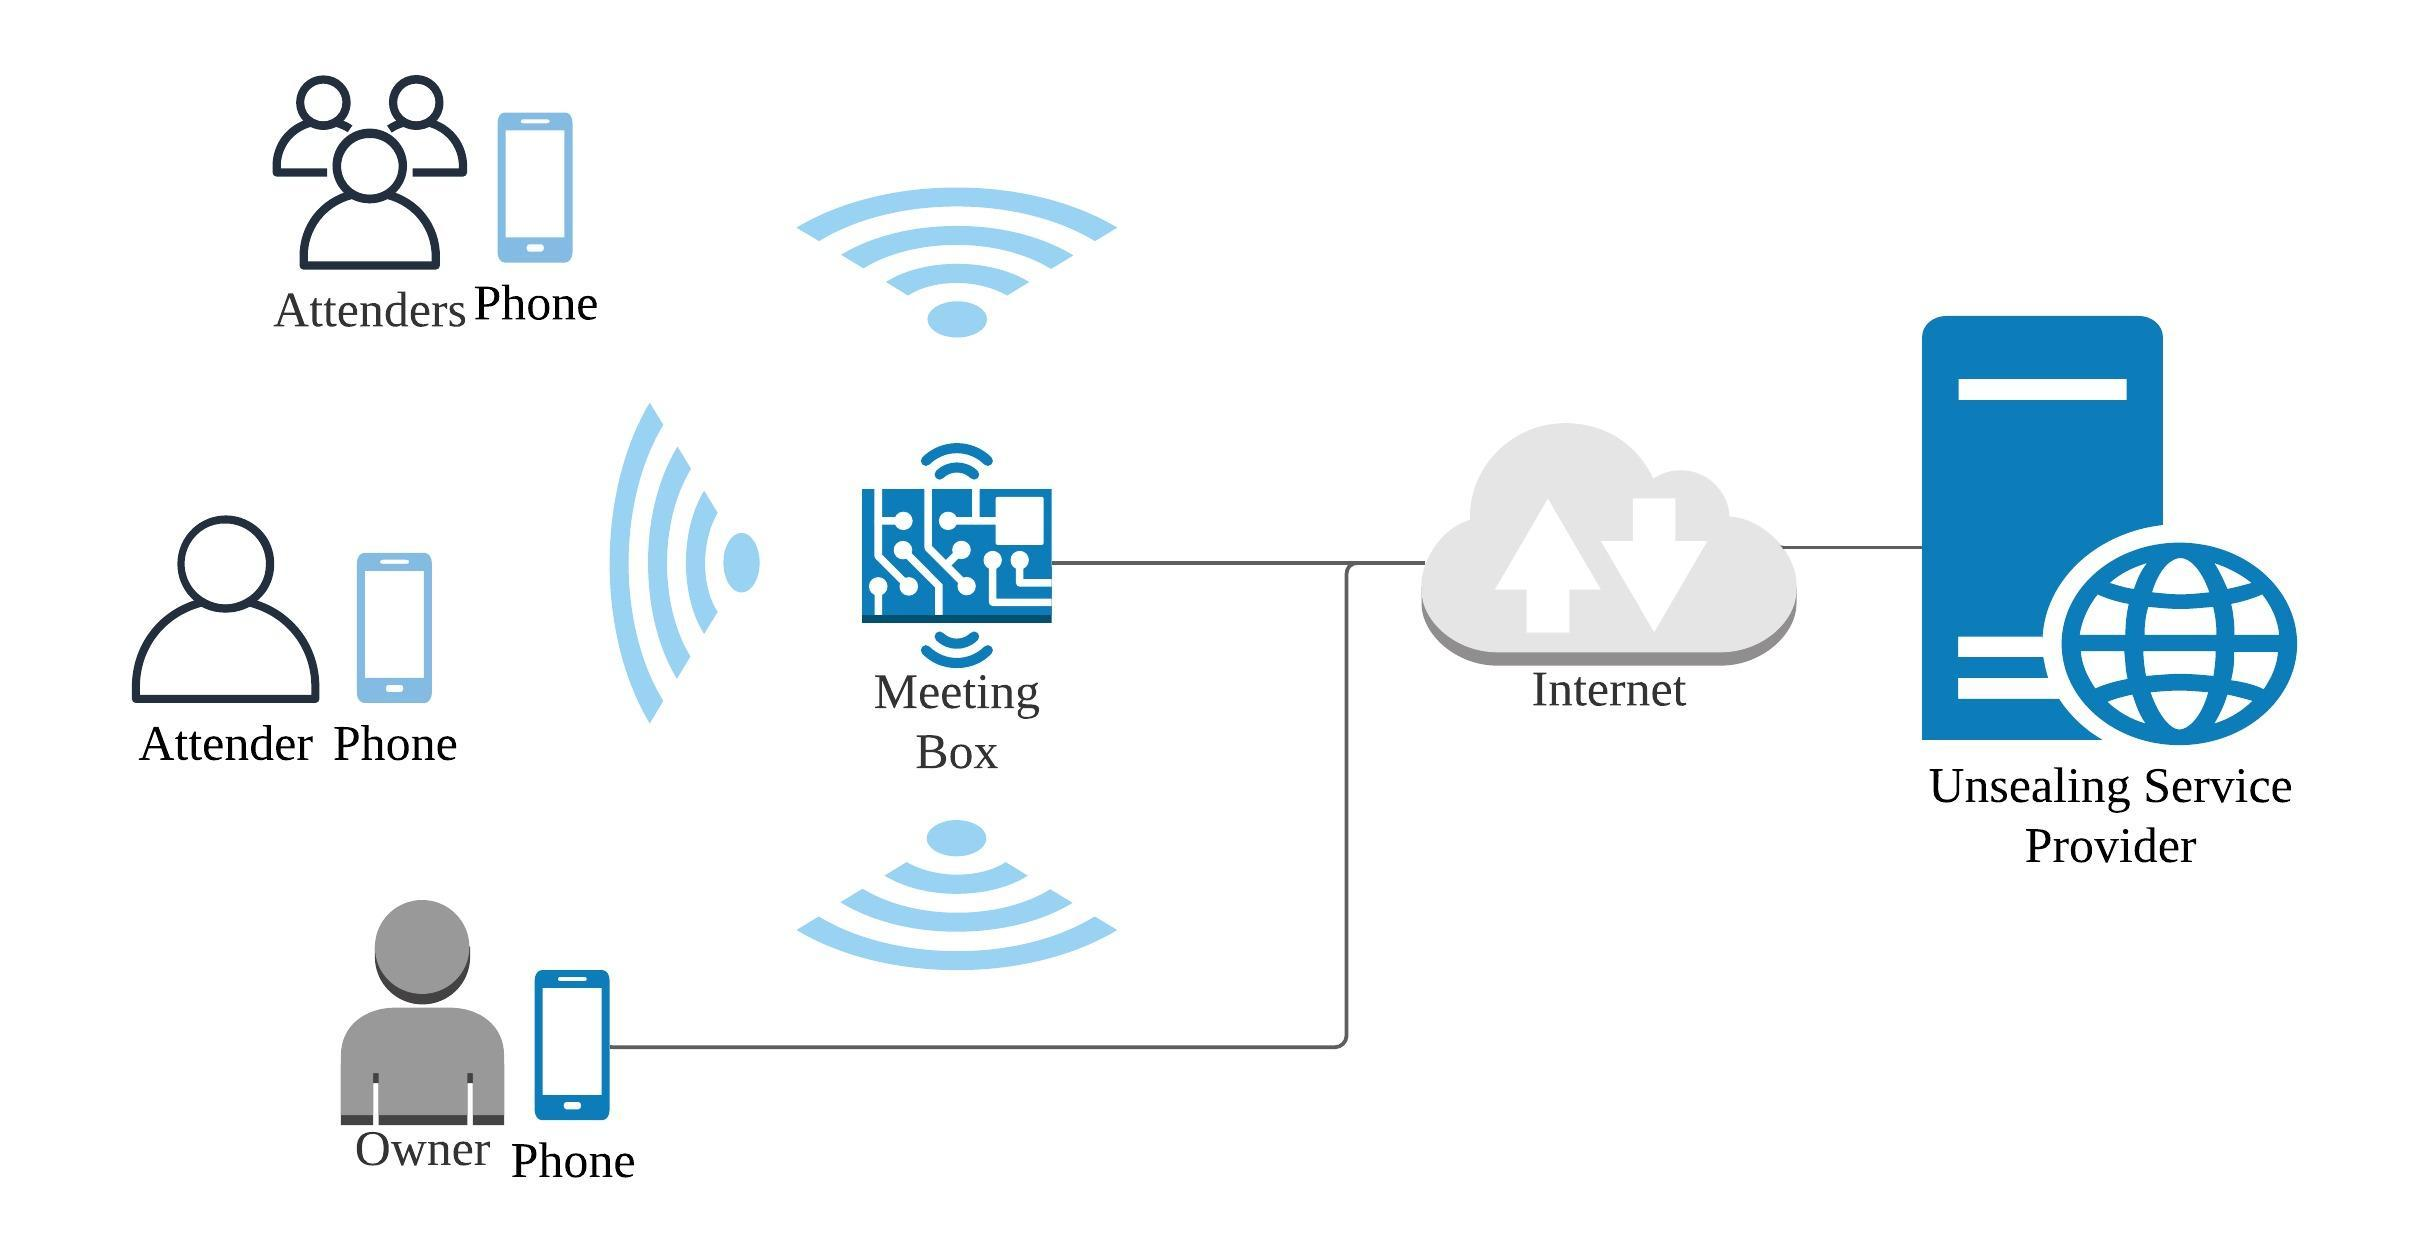
\includegraphics[width=0.7\textwidth]{single-owner-architecture}
    \caption{單一會談主持者情境圖}\label{fig:s-o-arch}
\end{figure}

    會談終端於會談進行中持續紀錄聲音,內容為受到超音波麥克風干擾器干擾的會談聲音記錄 (\DEFrecJ)。
於會談結束後,受干擾的會談聲音記錄 (\DEFrecJ),
將透過系統機制「解封會談聲音記錄」({\it Unsealing Session Record}),
使會談參與者中的會談主持者(Owner),獲得前述機制所產生的有效會談聲音記錄 (\DEFrecREV)。


\subsection{系統假設}

    本研究基於假設如下:

\begin{enumerate}
    \item 超音波麥克風干擾器產生顯著的干擾效果:

        近期的研究表明,目前的技術發展現狀已經能透過低成本、可穿戴式的裝置,
    產生有效的超音波麥克風干擾 \cite{chen2020demonstrating}。
    本研究實作嘗試復現 Yuxin Chen, Huiying Li 等人的實作 \cite{chen2020wearable},
    並透過復現實作的超音波麥克風干擾器作為為參考,近一步分析評估於不同信噪比時的干擾效果。
    如系統實驗 \ref{subsec:exp-jammer} \nameref{subsec:exp-jammer}。

    \item 系統各角色之間通訊為加密通道:

        目前的技術發展現狀,已經有成熟的技術可以為網路通訊創造一加密通道,
    提供通訊安全以保障資料的完整性、機密性。
    如傳輸層安全性協定(Transport Layer Security,TLS) \cite{rfc5246},
    在最新版本 TLS 1.3 中,更可以保障向前安全性 \cite{rfc8446}。
\end{enumerate}


\subsection{會談參與者}

    會談參與者(Attender) 為一集合,代表所有當次會談 ({\it Meeting Session}) 的所有參與者。
會談參與者包含會談主持者(Owner),為會談主持者的超集合。其餘非會談主持者的會談參與者視為一般參與者。
會談參與者透過會談終端上的控制介面與其互動,進而控制會談的生命週期。

    於會談進行中,會談參與者受到會談終端中的超音波麥克風干擾器的干擾,使得隨身的麥克風或聲音記錄裝置,
都將因受到干擾而失效,無法有效記錄會談內容。例如:智慧型手機、智慧手錶、筆電、平板、智慧喇叭等。


\subsection{會談主持者}

    會談主持者(Owner),屬於會談參與者(Attender),為會談參與者的子集合,定義為會談參與者中的特權角色。
會談主持者如未執行本研究所設計的系統機制「註冊會談主持者」 (Register Owner),則視為一般參與者。
於會談 ({\it Meeting Session}) 結束後,
會談主持者有能力決定是否執行系統機制「解封會談聲音記錄」({\it Unsealing Session Record}),
並獲取解封會談聲音記錄後所產生的有效會談聲音記錄 (\DEFrecREV)。

    會談主持者可以是一或多人。當會談中只有一個會談主持者時,為「單一會談主持者」情境,
系統架構如圖 \ref{fig:s-o-arch}。當會談中多於一個會談主持者時,為「多會談主持者」情境,
系統架構如圖 \ref{fig:m-o-arch} 所示。

    會談主持者持有智慧型裝置,且透過 App 與會談終端互動,獲取會談終端上的資訊。
並同樣有能力於會談進行中、談結束後,與解封伺服器進行通訊。

\begin{figure}[H]
    \centering
    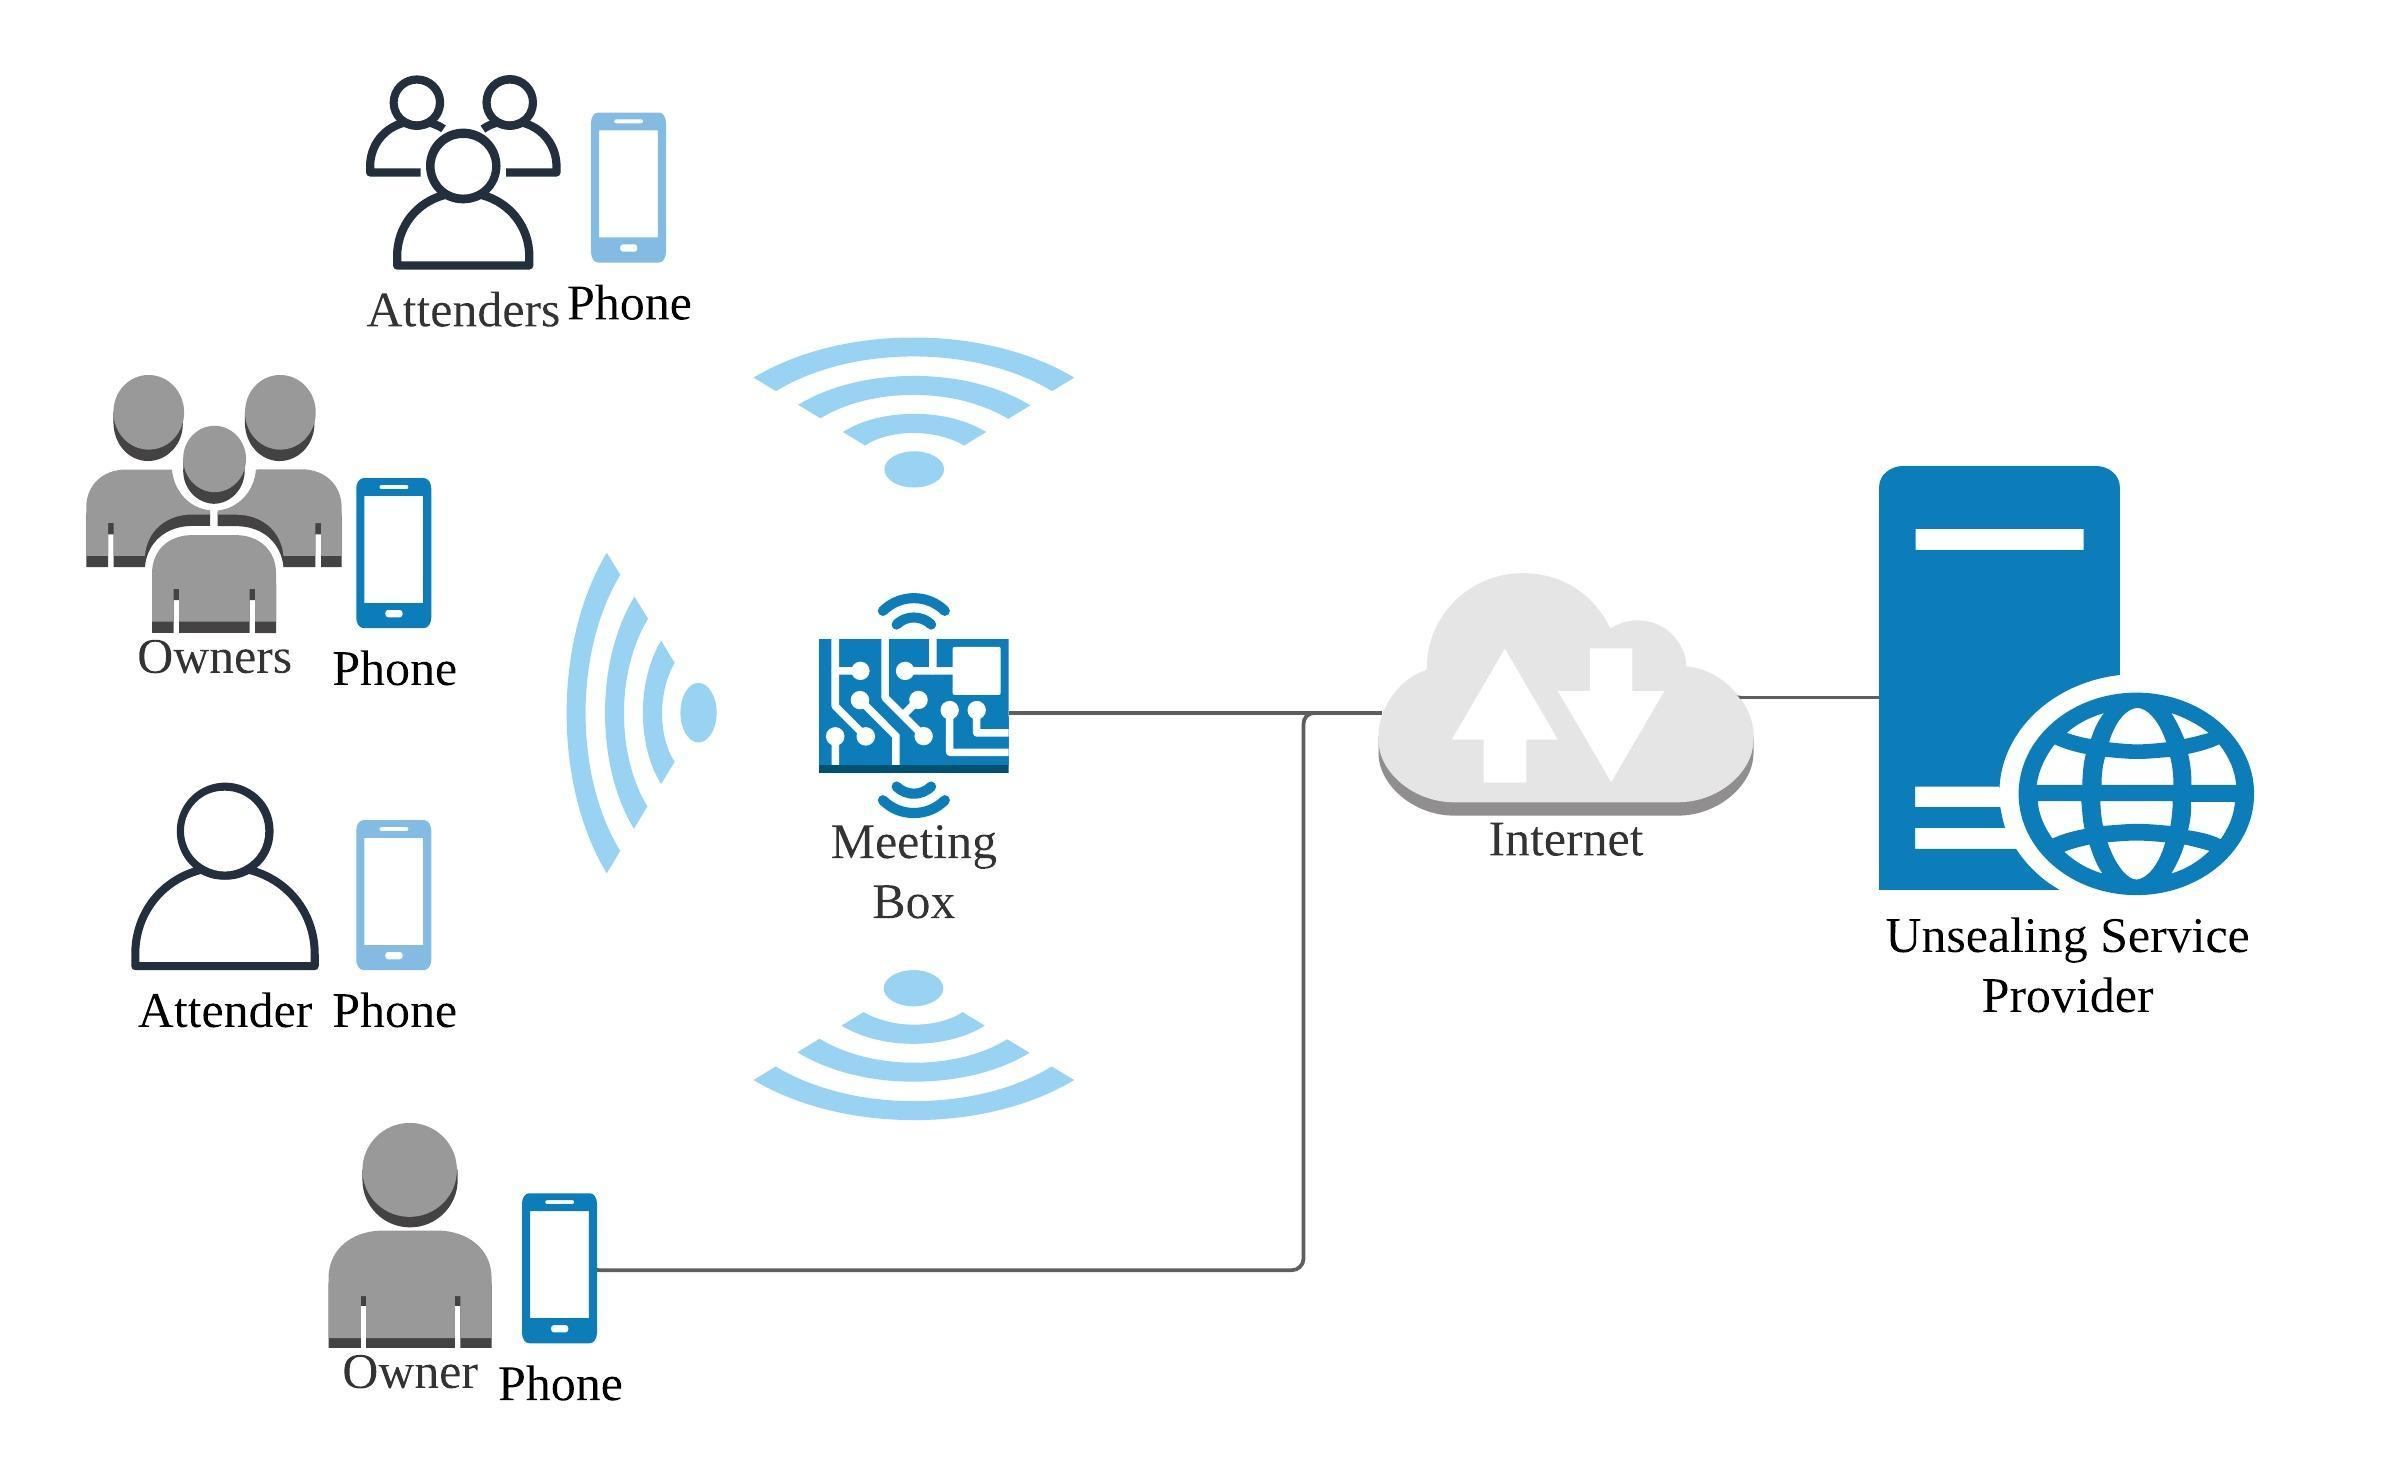
\includegraphics[width=0.8\textwidth]{multi-owner-architecture}
    \caption{多會談主持者情境圖}\label{fig:m-o-arch}
\end{figure}


\subsection{會談終端}

    會談終端(MeetingBox),定義符號為 \DEFmeetingbox 。
會談終端部署於會談 ({\it Meeting Session}) 的場域,與會談參與者(Attender)實體接觸,
透過與會談參與者的互動,成為觸發會談生命週期改變事件的控制核心,同時也作為系統聲音紀錄的輸入來源。
故一組會談終端僅能同時間處理一場會談的進行。

    會談終端包含多個組件,如下所列:

    \begin{enumerate}
        \item 超音波麥克風干擾器:\\
            使用偽隨機數產生器 \DEFfuncPRNG{} 產生亂數頻率的超音波,於會談進行中開啟。
            用於干擾鄰近周圍含有麥克風的裝置,使其無法有效記錄會談內容。
            \DEFfuncPRNG{} 的輸入為亂數種子 \DEFseed。

        \item 錄音麥克風:\\
            用於錄製受超音波麥克風干擾器干擾的會談對話聲音記錄 (\DEFrecJ),
            與產生純超音波麥克風干擾器於麥克風的響應輸出(純噪音)之聲音記錄 (\DEFrecN)。

        \item 物理控制介面:\\
            提供會談參與者操作與會談終端互動,獲得外部觸發事件。

        \item 人機互動介面:\\
            用於傳遞會談的元資料與系統狀態提示給會談主持者與提示系統狀態給會談參與者。

        \item 運算控制核心與網路介面:\\
            周邊裝置控制與邏輯運算核心,用於處理聲音記錄、執行加密與解封伺服器通訊等運算工作。
    \end{enumerate}


\subsection{解封伺服器}

    解封伺服器(Unsealing Service Provider),定義符號為 \DEFserver。
解封伺服器可部署於雲端,不需實體與會談參與者(Attender)接觸。
透過會談主持者(Owner)向解封伺服器註冊與授權實現存取控制,目標為取得產生效之會談聲音記錄 \DEFrecREV。
解封伺服器之設計能與多個會談終端(MeetingBox)配合,同時間處理一場以上的會談 ({\it Meeting Session}) 的進行。


\section{系統流程}\label{sec:system-flow}

    本研究所設計之系統,其流程跟隨會談 ({\it Meeting Session}) 的生命週期,其分為三個階段定義。分別為:
一、「初始化會談 (Initialize Meeting Session)」;
二、「進行會談 (Running Meeting Session)」;
三、「解封會談聲音記錄」(Unsealing Session Record)」;
如圖 \ref{fig:system-stage}。

\begin{figure}[H]
    \centering
    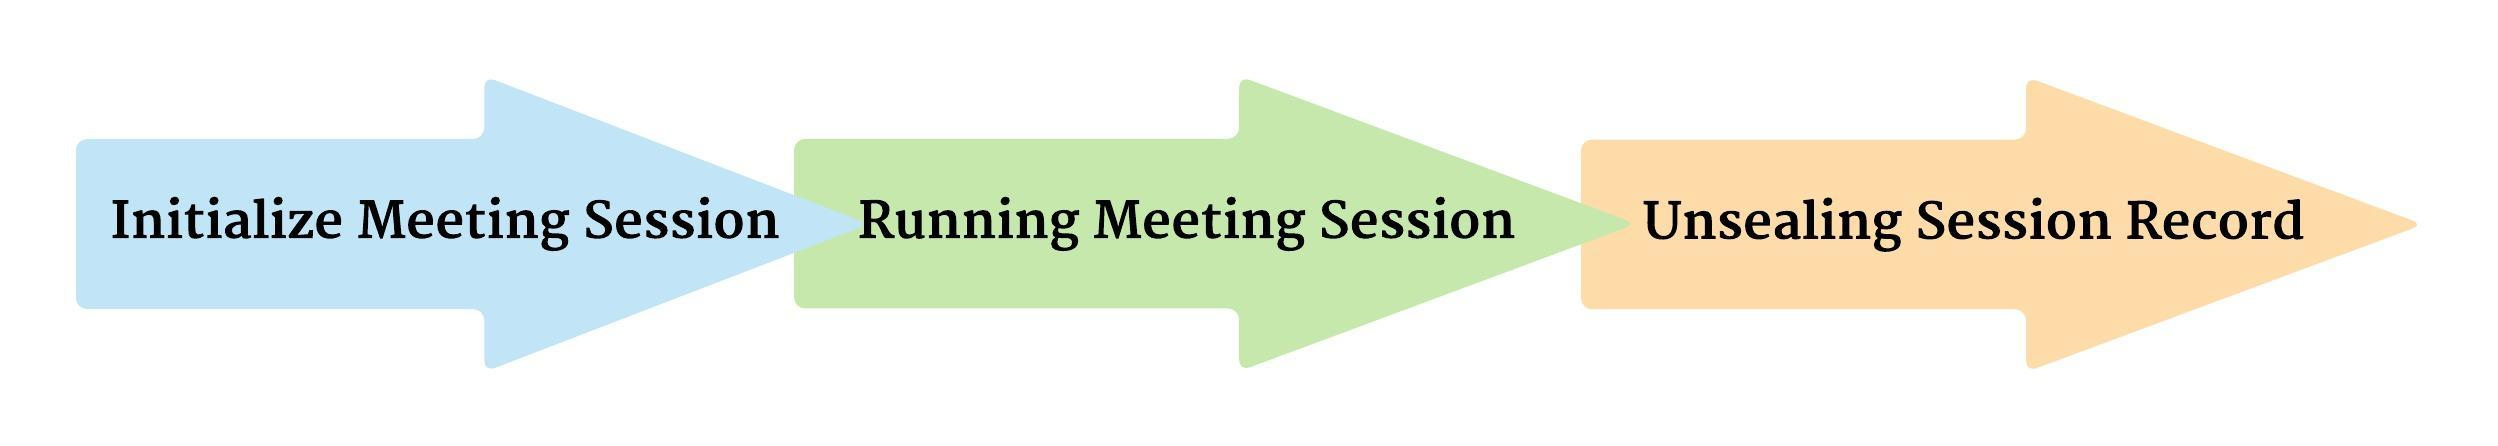
\includegraphics[width=0.7\textwidth]{system-stage}
    \caption{會談生命週期}\label{fig:system-stage}
\end{figure}

    本章節將介召會談生命週期各階段的流程步驟。
第一階段為會談的起始點,各階段依序執行,於第三階段結束,完成一次系統生命週期的循環。
透過解封伺服器與多個會談終端配合,系統可以同時存在多個會談生命週期,彼此互不干擾,獨立執行。
依據會談主持者的數量,將分為兩種情境說明討論:
一、「單一會談主持者情境 ({\it Single Owner})」;
二、「多會談主持者情境 ({\it Multi Owner})」;
當會談參與者裡僅有一位會談主持者,為單一會談主持者情境,若會談中多於一個會談主持者時,則為多會談主持者情境。

    接續章節將首先說明,於單一會談主持者情境中的流程與步驟。


\subsection{初始化會談}\label{subsec:initialize}

    此章節將說明於單一會談主持者 ({\it Single Owner}) 情境中,
會談生命週期第一個階段「初始化會談 (Initialize Meeting Session)」的系統流程。
如圖 \ref{fig:s-o-init} 所示。

\begin{figure}[H]
    \centering
    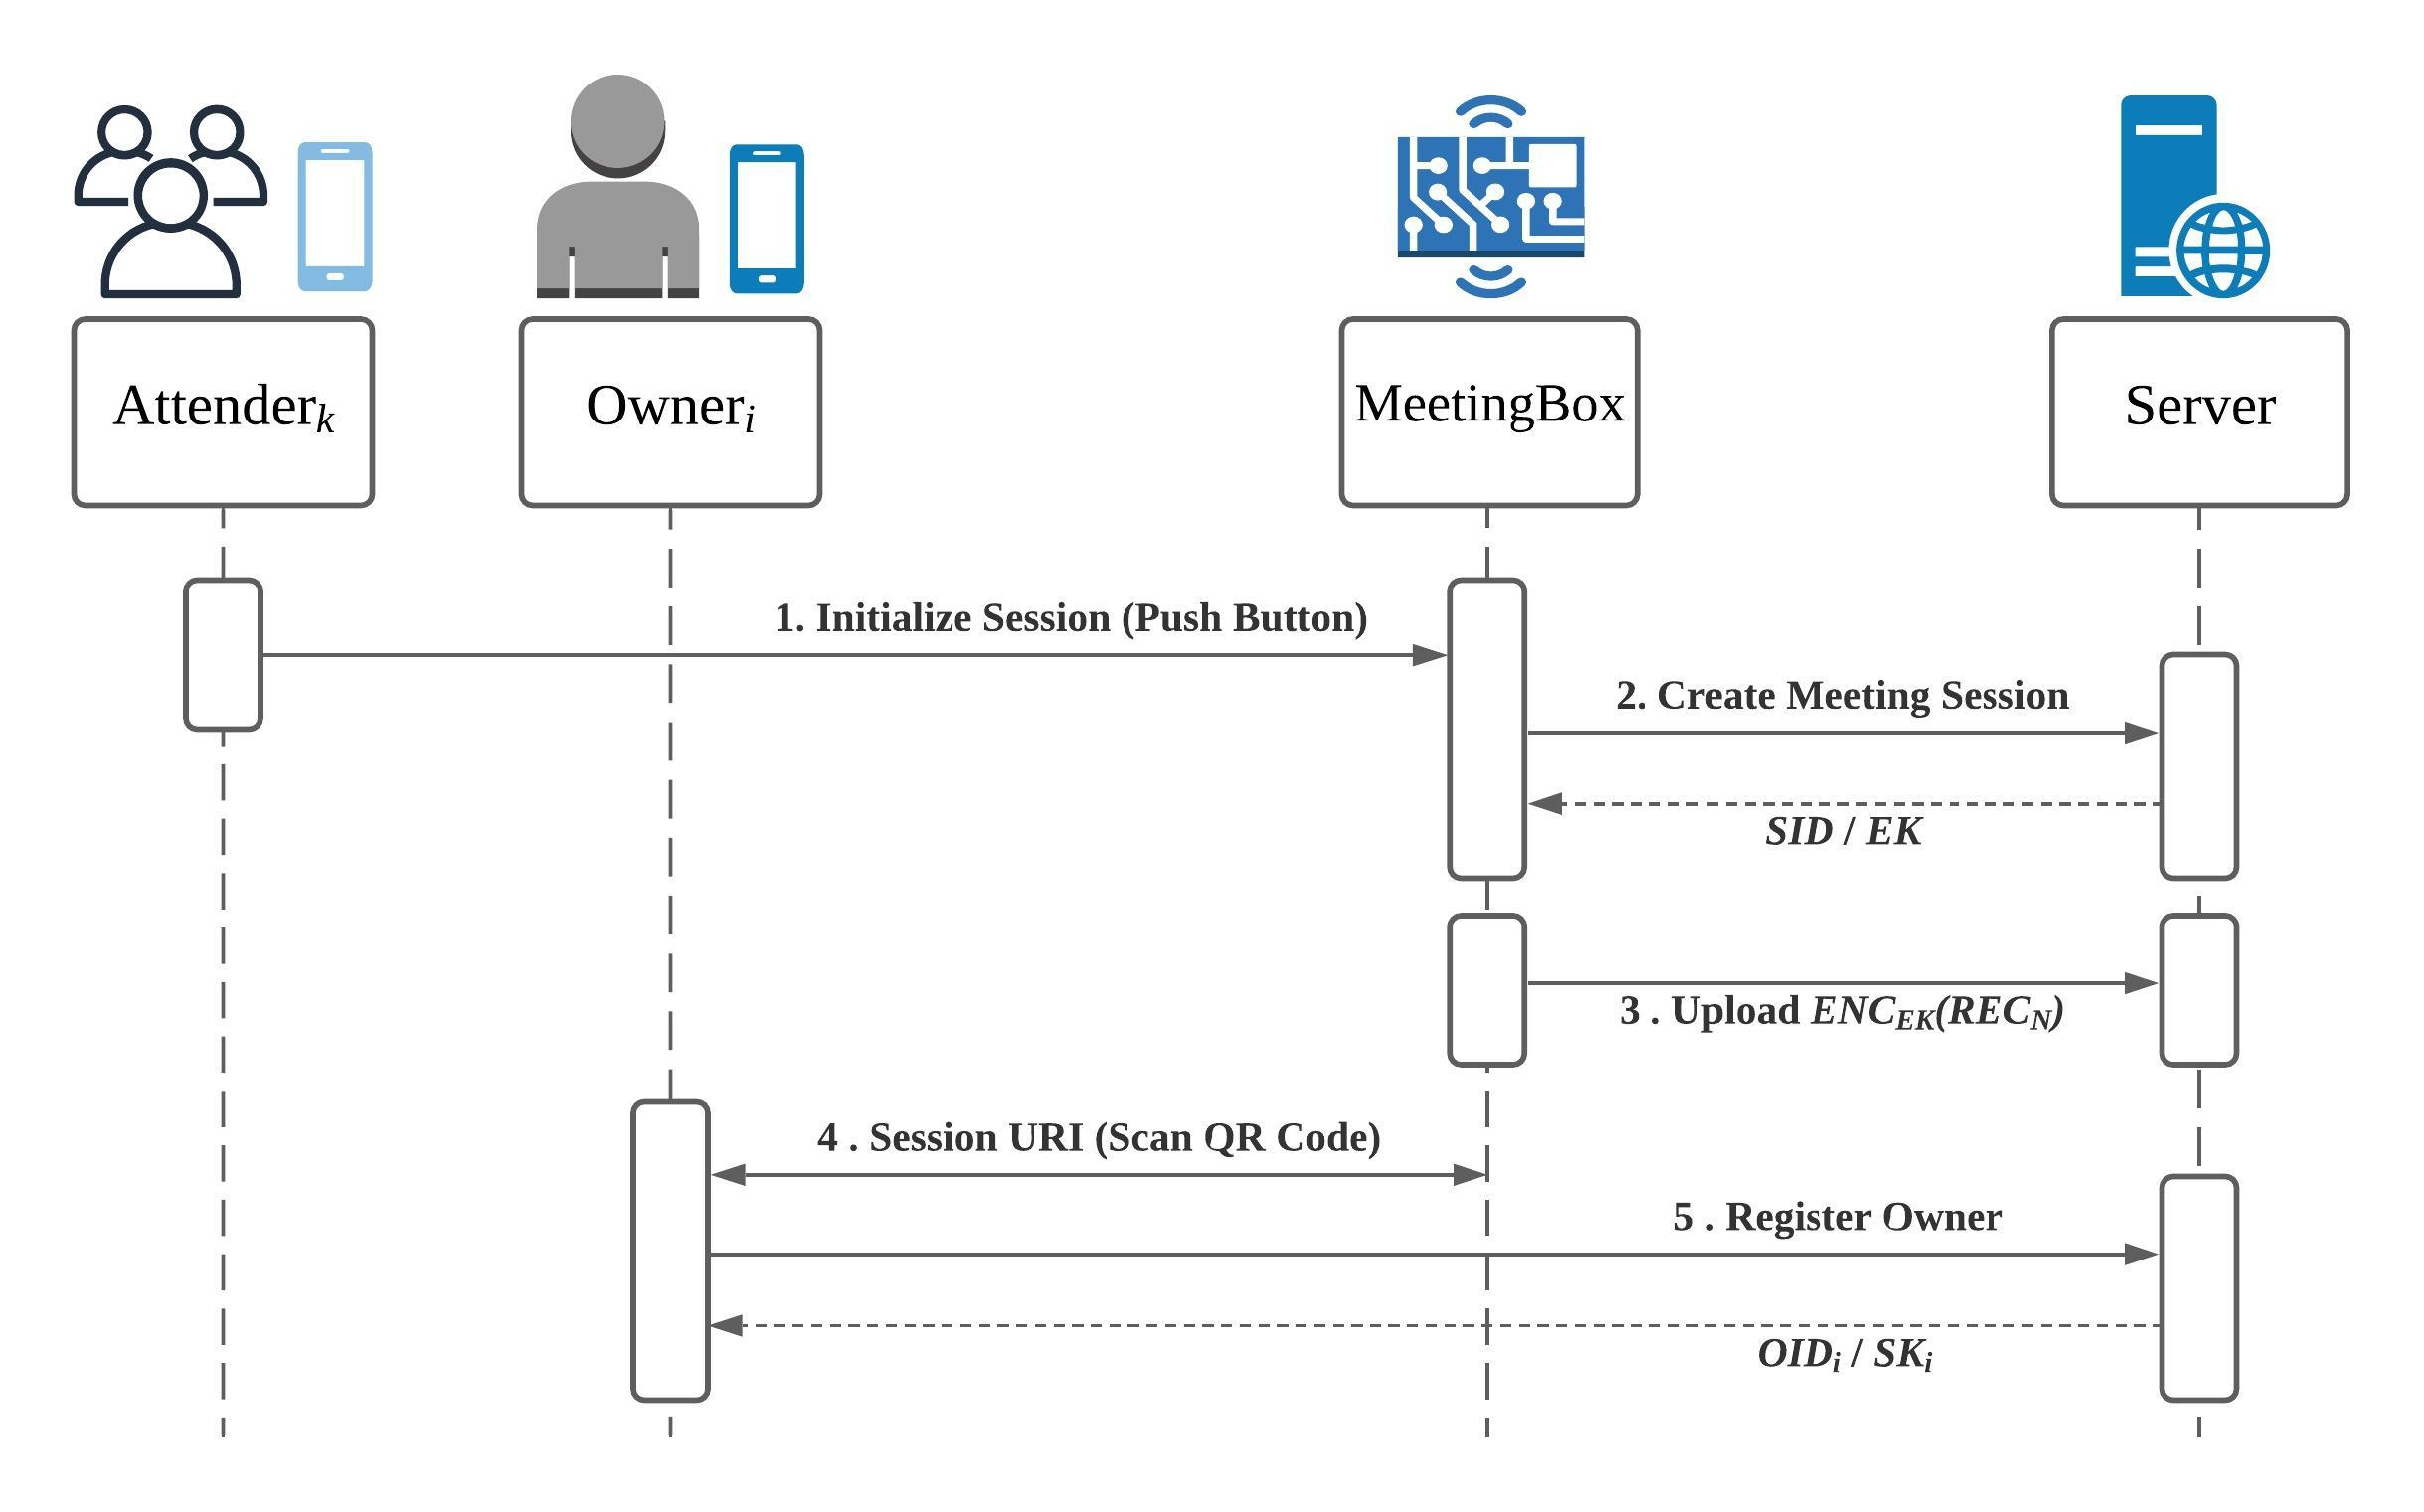
\includegraphics[width=0.8\textwidth]{single-owner-sequence-diagram-init}
    \caption{初始化會談於單一會談主持者情境}\label{fig:s-o-init}
\end{figure}

\begin{steps}
    \item 建立會談(Create Meeting Session):

            會談參與者在欲進行會談會談終端 \DEFmeetingbox 的周圍準備開始會談,
        會談參與者透過控制會談終端上的物理控制介面,使會談終端獲得外部事件,觸發建立會談。

    \item 初始化會談(Initialize Meeting Session):

            會談終端觸發建立會談後,
        首先對解封伺服器 \DEFserver 傳送請求初始化會談。
        會談終端透過解封伺服器的回覆獲取本次會談的元資料與加密金鑰。

    \item 上傳受加密保護的噪音(Upload Encrypted Noise):

            使用加密金鑰加密預先配置存在於會談終端 \DEFmeetingbox 的純噪音之聲音記錄,
        並上傳至解封伺服器 \DEFserver。

    \item 取得會談資源位置(Get Session URI):

            會談主持者透過會談終端 \DEFmeetingbox 上的人機互動介面,
        取得此次會談的元資料與封伺服器的資源位置 URI (Uniform Resource Identifier)。

    \item 註冊會談主持者(Register Owner):

            會談主持者透過取得的會談元資料與資源位置,向解封伺服器 \DEFserver 請求註冊。
        註冊成功則成為此次會談的會談主持者,並取得代表會談主持者身份的私密金鑰。
\end{steps}

\subsection{進行會談}\label{subsec:sessioning}

    此章節將說明於單一會談主持者 ({\it Single Owner}) 情境中,
會談生命週期第二個階段「進行會談 (Running Meeting Session)」的系統流程。
如圖 \ref{fig:s-o-sessioning} 所示。

\begin{figure}[H]
    \centering
    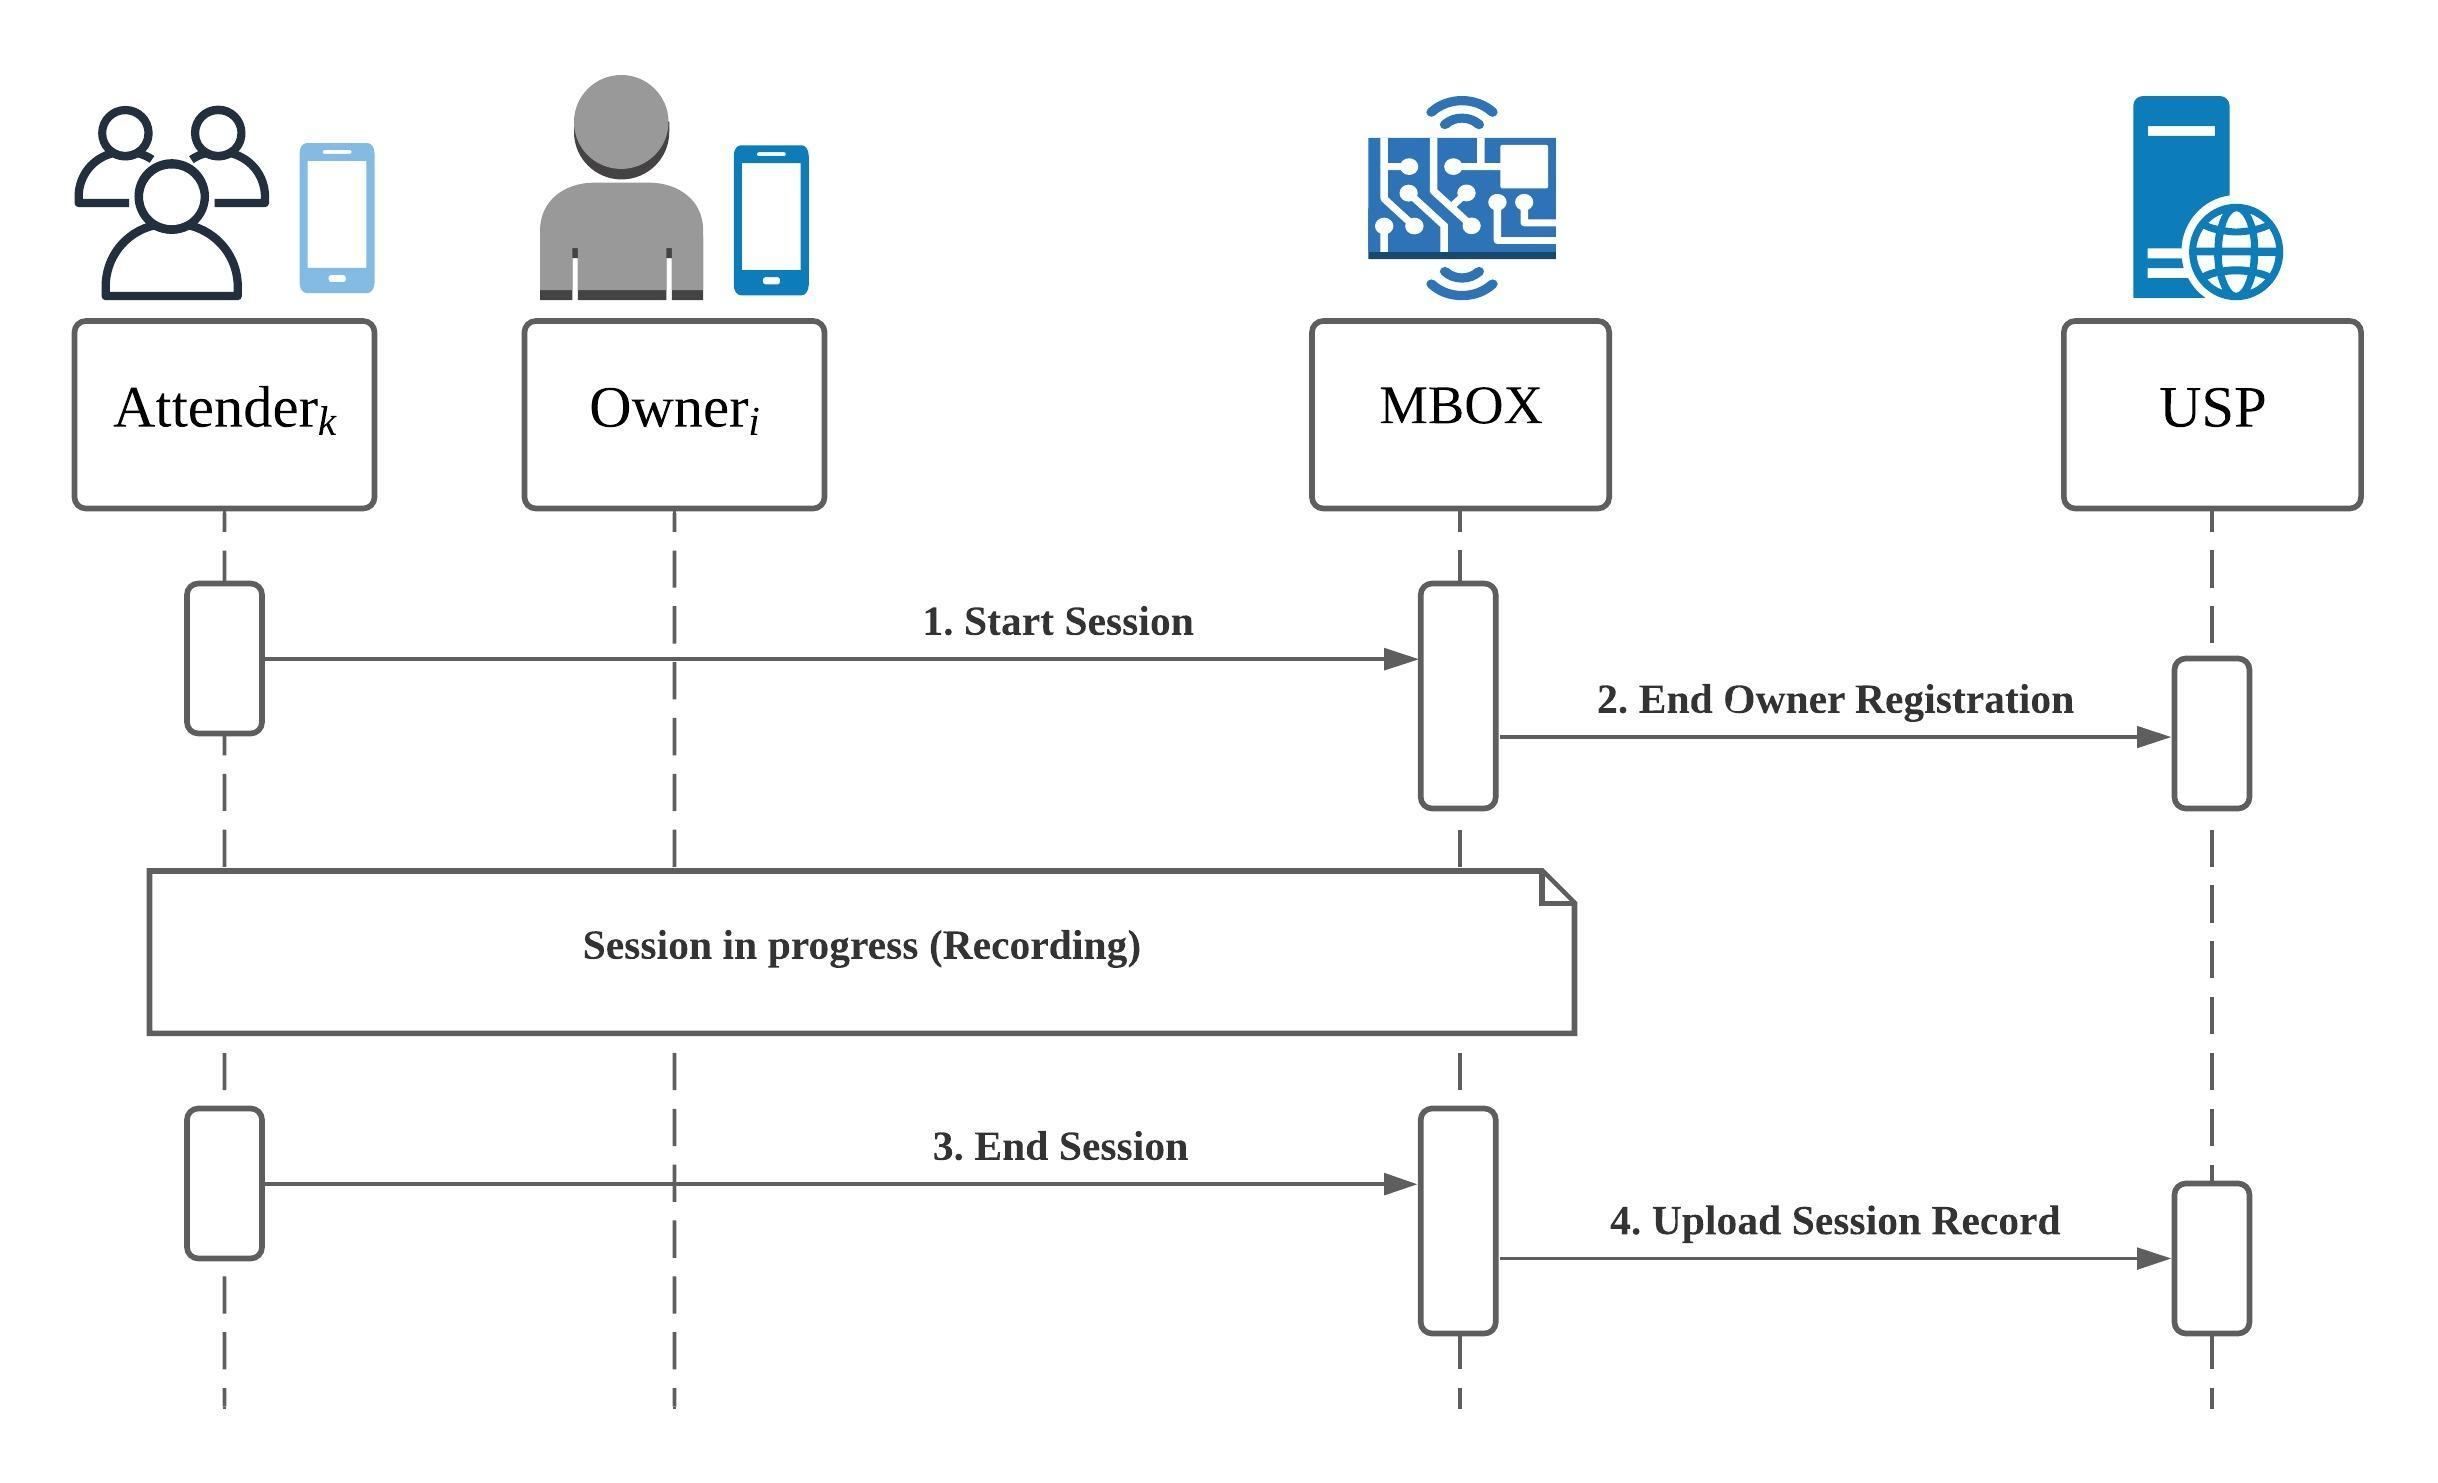
\includegraphics[width=0.8\textwidth]{single-owner-sequence-diagram-sessioning}
    \caption{進行會談於單一會談主持者情境}\label{fig:s-o-sessioning}
\end{figure}

\begin{steps}
    \item 開始會談(Start Session):

            會談參與者透過控制會談終端上的物理控制介面,
        使會談終端 \DEFmeetingbox 獲得外部事件,觸發開始會談。

    \item 終止會談主持者註冊(End Owner Registration):

            會談終端 \DEFmeetingbox 向解封伺服器 \DEFserver 發起請求,
        通知解封伺服器,會談主持者的註冊已完成。

            隨後開啟會談終端上的麥克風與麥克風超音波干擾器,並透過人機互動介面提示系統已經開始錄音。

            因超音波麥克風干擾器的干擾,場域內的任何錄音將成為非有效之聲音記錄。
        此時會談參與者即可進行私密會談,不用擔心存在其他麥克風或聲音記錄裝置可以取得有效之聲音記錄。

    \item 結束會談(End Session):

            當會談對話結束時,會談參與者即可透過會談終端 \DEFmeetingbox 的物理控制介面,
        使會談終端獲得外部事件,觸發結束會談。

            會談終端此時關閉麥克風與超音波麥克風干擾器,人機互動介面同時提示系統已結束錄音。
        此階段所錄製的聲音記錄內容為音波麥克風干擾器與會談聲音內容的疊加,同為非有效之聲音記錄。

    \item 上傳會談聲音紀錄(Upload Session Record):

            隨後會談終端 \DEFmeetingbox 將為受干擾的會談聲音記錄上傳至解封伺服器 \DEFserver。
        此時會談參與者即可離開會談場域,不再需要與會談終端實體接觸。
\end{steps}


\subsection{解封會談聲音記錄}\label{subsec:unseal}

    此章節將說明於單一會談主持者 ({\it Single Owner}) 情境中,
會談生命週期第三個階段「解封會談聲音記錄」(Unsealing Session Record)」的系統流程。
如圖 \ref{fig:s-o-unseal} 所示。

\begin{figure}[H]
    \centering
    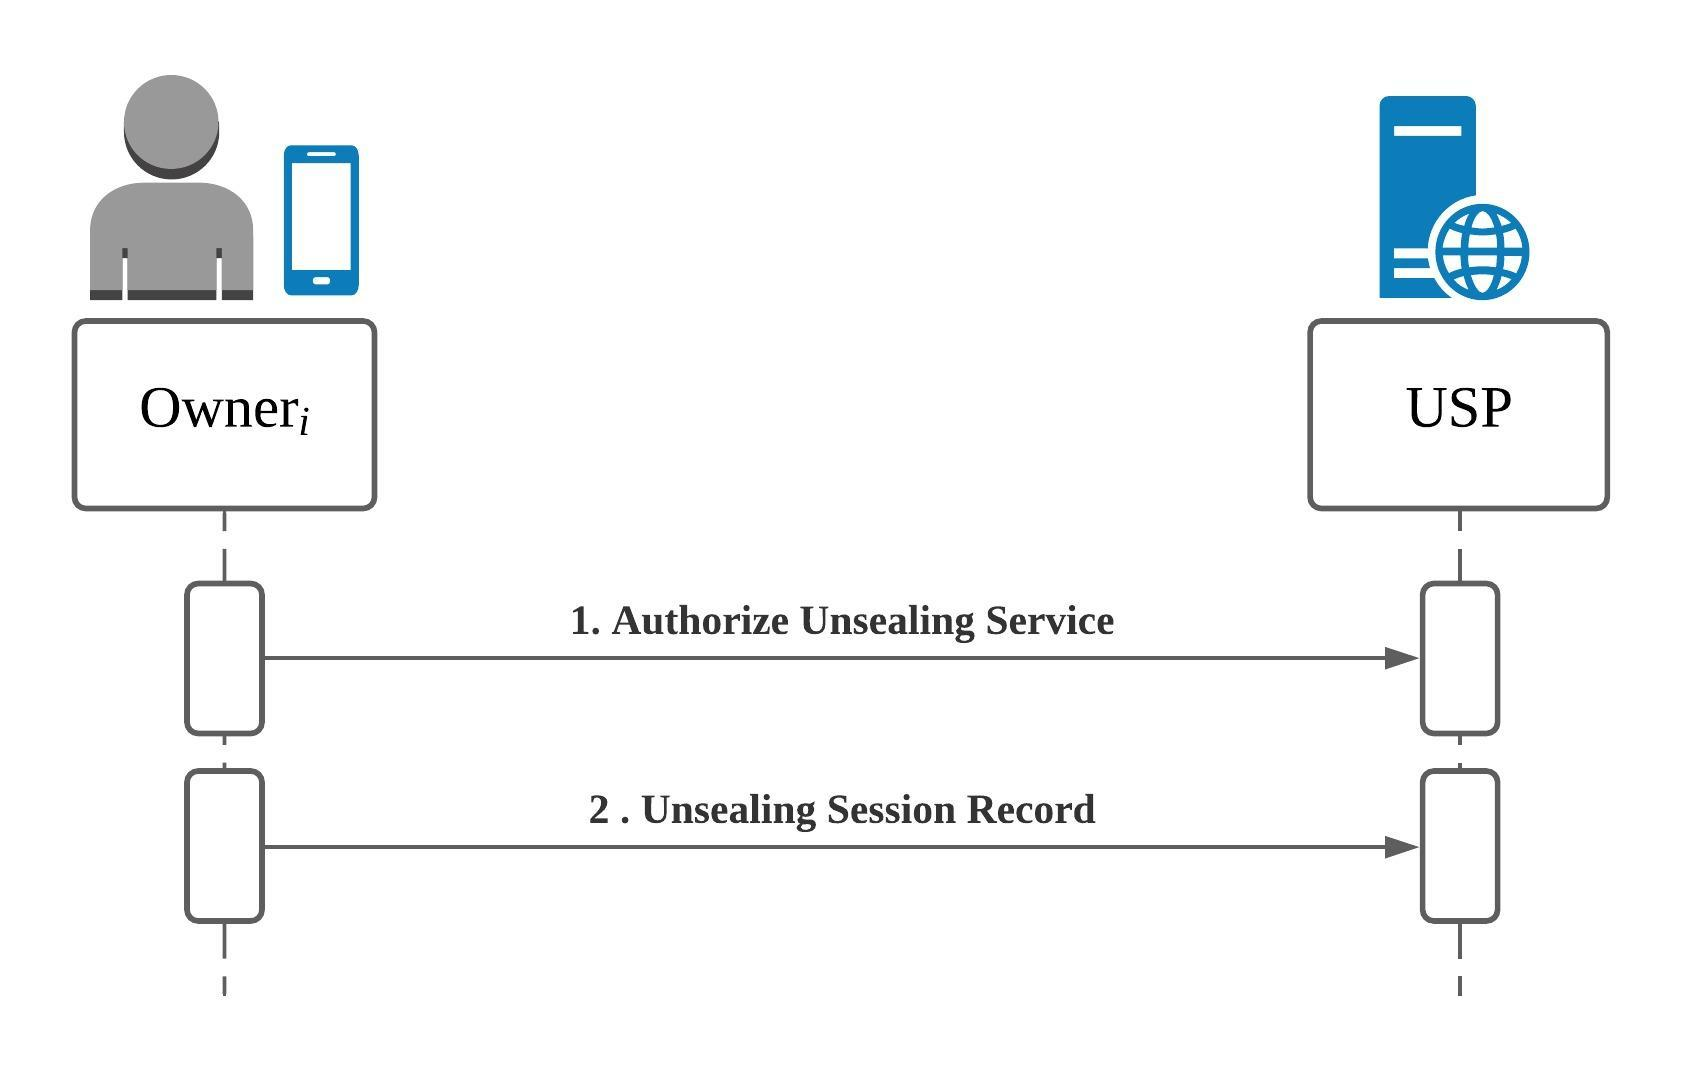
\includegraphics[width=0.6\textwidth]{single-owner-sequence-diagram-unseal}
    \caption{解封會談聲音記錄於單一會談主持者情境}\label{fig:s-o-unseal}
\end{figure}

\begin{steps}
    \item 授權解封伺服器(Authorize Unsealing Service):

            在會談對話結束後,會談主持者欲取得當時會談的有效聲音紀錄,須先授權解封伺服器 \DEFserver。

            此時會談主持者向解封伺服器發起授權請求,
        並透過代表會談主持者身份的私密金鑰,證明會談主持者的身份與授權解封伺服器。

    \item 存取會談聲音記錄(Access Session Record):

            在會談主持者成功授權解封伺服器 \DEFserver 後,向解封伺服器發起請求取得有效之會談聲音記錄。

            此時封伺服器將受加密保護的純噪音之聲音記錄解密,
        與含有噪音的受干擾會談聲音記錄透過自適應噪音消除,還原出有效之會談聲音記錄。
        最終使會談主持者取得此有效之會談聲音記錄。
\end{steps}


\subsection{多會談主持者情境}

    此章節將說明於多會談主持者 ({\it Multi Owner}) 情境中,系統生命週期階段的流程步驟。
當存在會談中會談主持者數量為二人以上,即定義為多會談主持者情境。

    於此情境中,會談生命週期與前篇單一會談主持者 ({\it Single Owner}) 情境相似。
其差異之處在於會談主持者數量大於二人。基於單一會談主持者情境,僅需小幅度的系統改動,即可達成多會談主持者情境。

    多會談主持者 ({\it Multi Owner}) 情境中,
會談生命週期第三個階段「解封會談聲音記錄」(Unsealing Session Record)」的系統流程。
如圖 \ref{fig:m-o-init} 所示。

\begin{figure}[H]
    \centering
    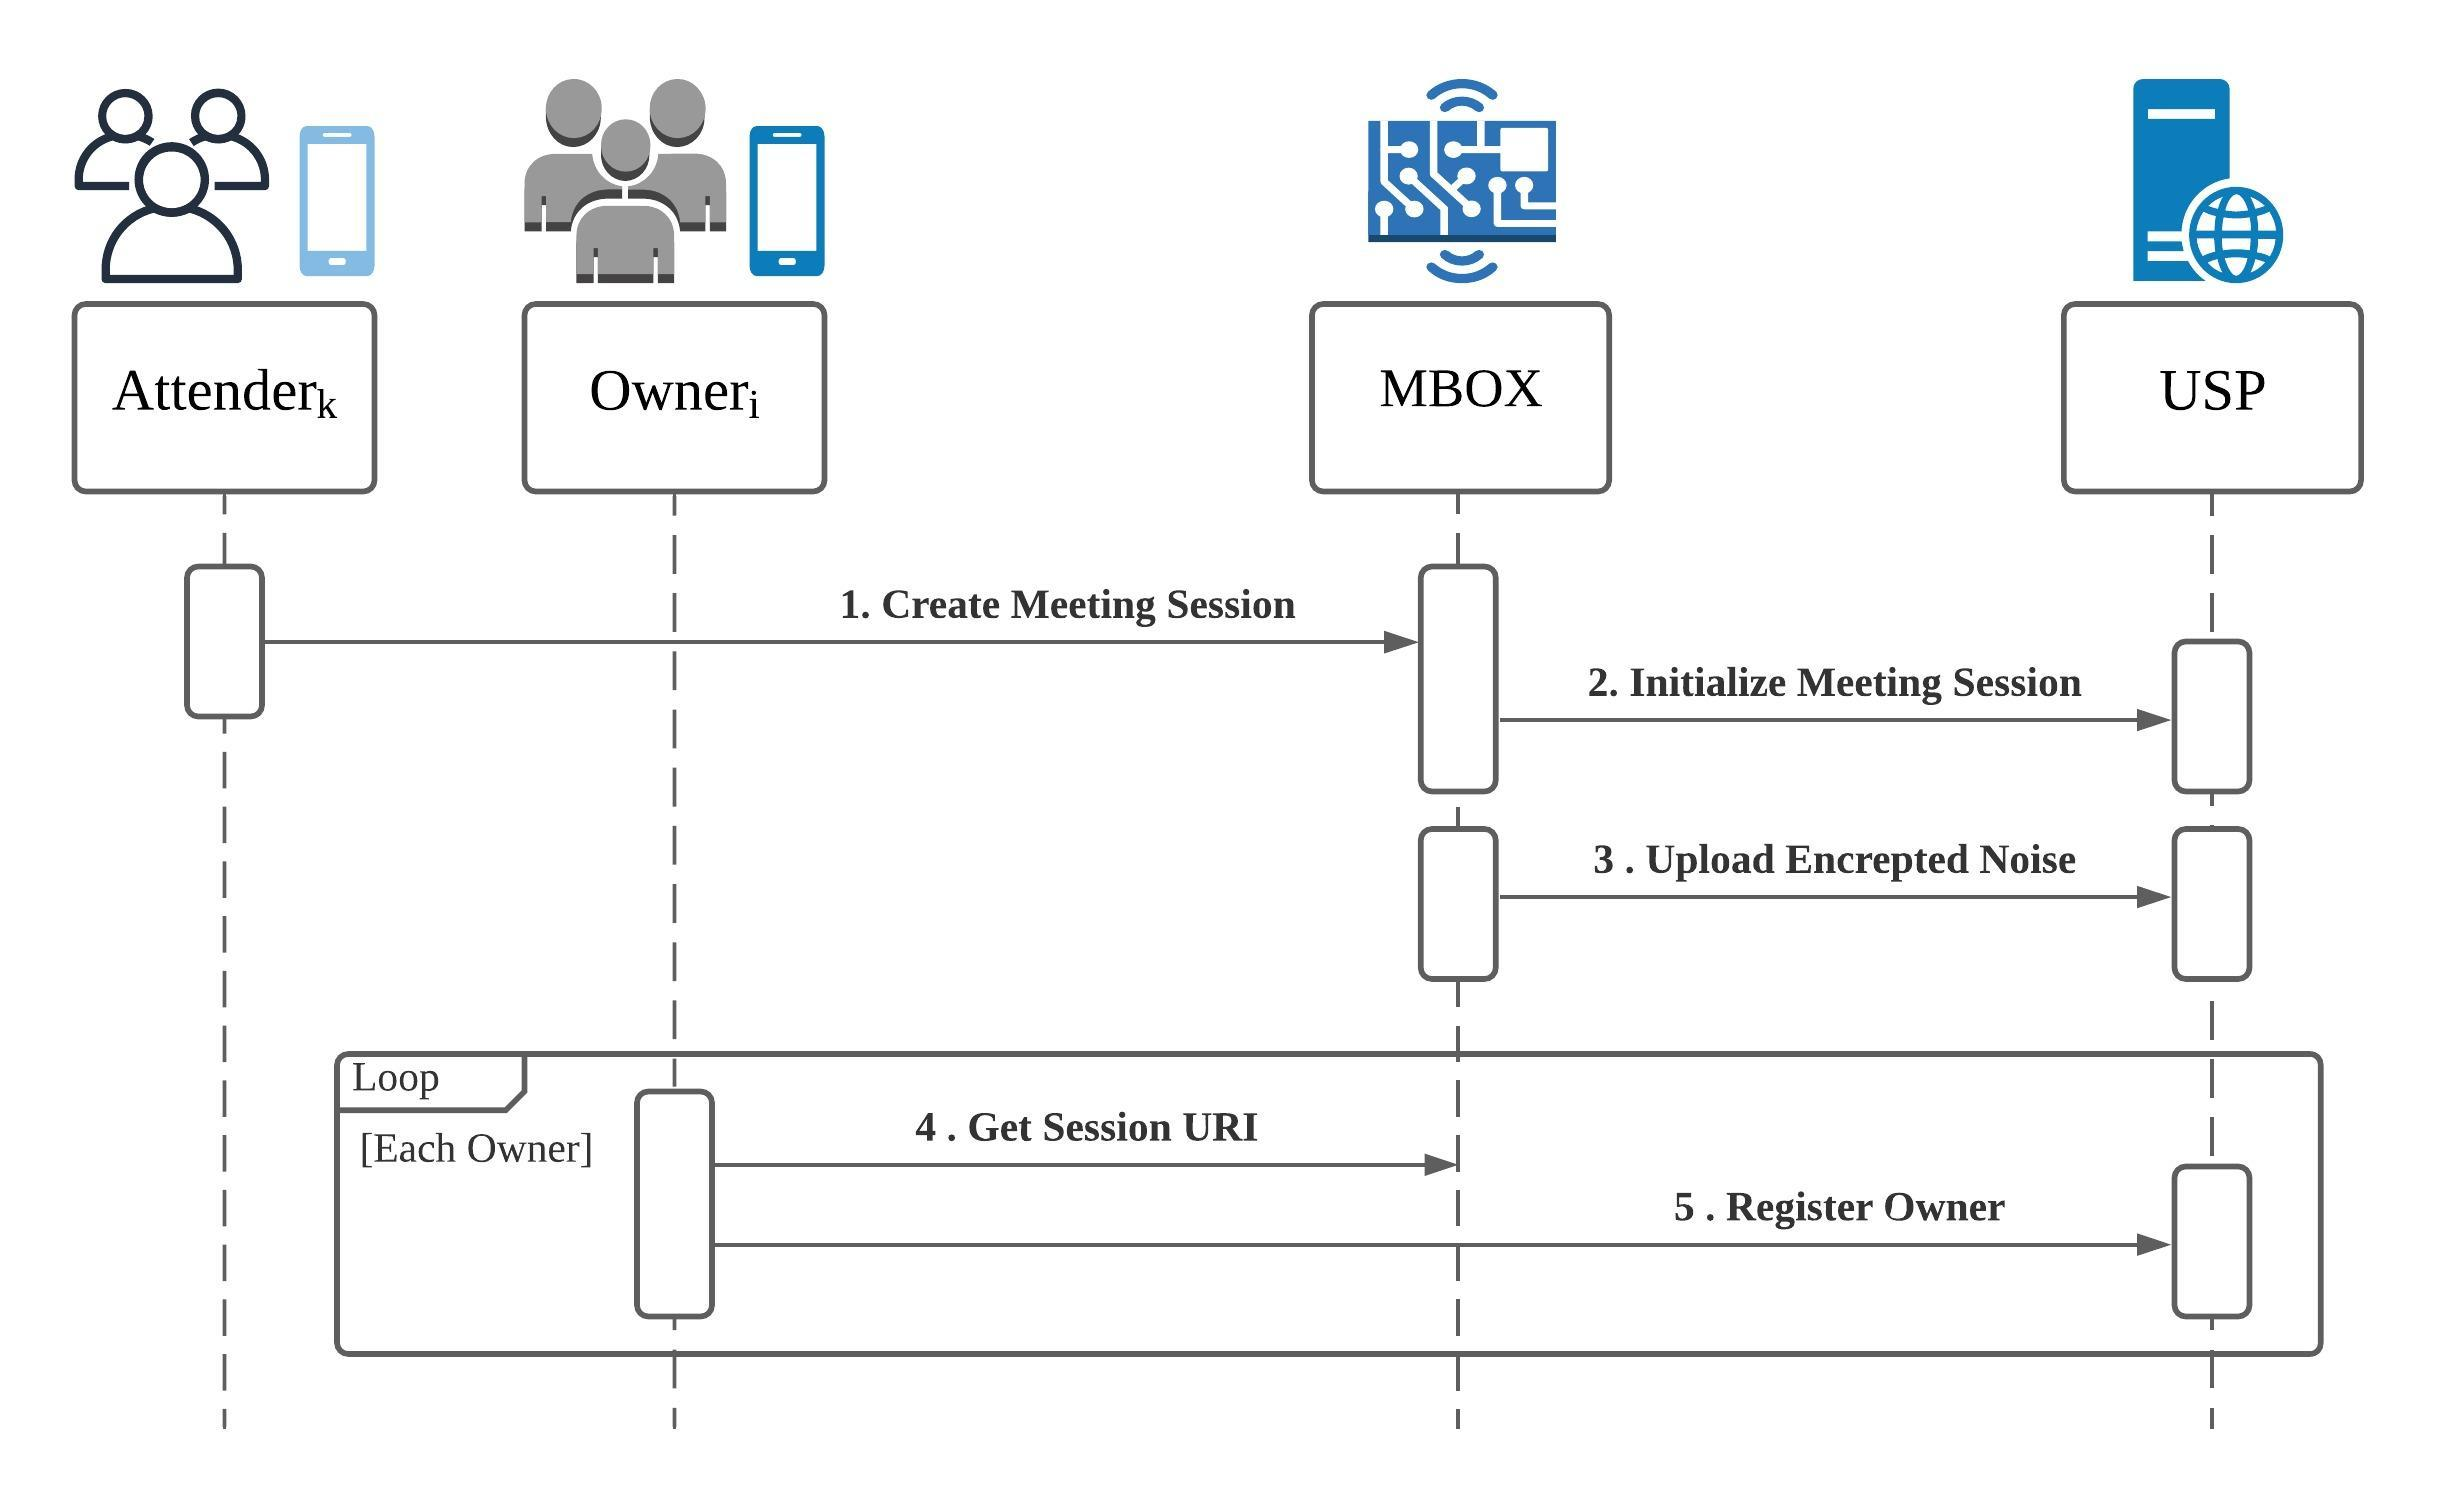
\includegraphics[width=0.8\textwidth]{multi-owner-sequence-diagram-init}
    \caption{初始化會談於多會談主持者情境}\label{fig:m-o-init}
\end{figure}

    圖中步驟 1\textasciitilde3 與 \ref{subsec:initialize} \nameref{fig:s-o-init} 中的流程步驟相同。
其中步驟 4\textasciitilde5 需要所有的會談主持者 \DEFownerAll 中的每一位會談主持者 \DEFowner 執行完成。
各會談主持者 \DEFowner 可以同時獨立執行,每個會談主持者 \DEFowner 的執行結果不受其他會談主持者影響。
待所有 \DEFowner 執行成功,即完成此階段。

    於多會談主持者 ({\it Multi Owner}) 情境中,
會談生命週期第二個階段「進行會談 (Running Meeting Session)」的系統流程。
如圖 \ref{fig:m-o-sessioning} 所示。

\begin{figure}[H]
    \centering
    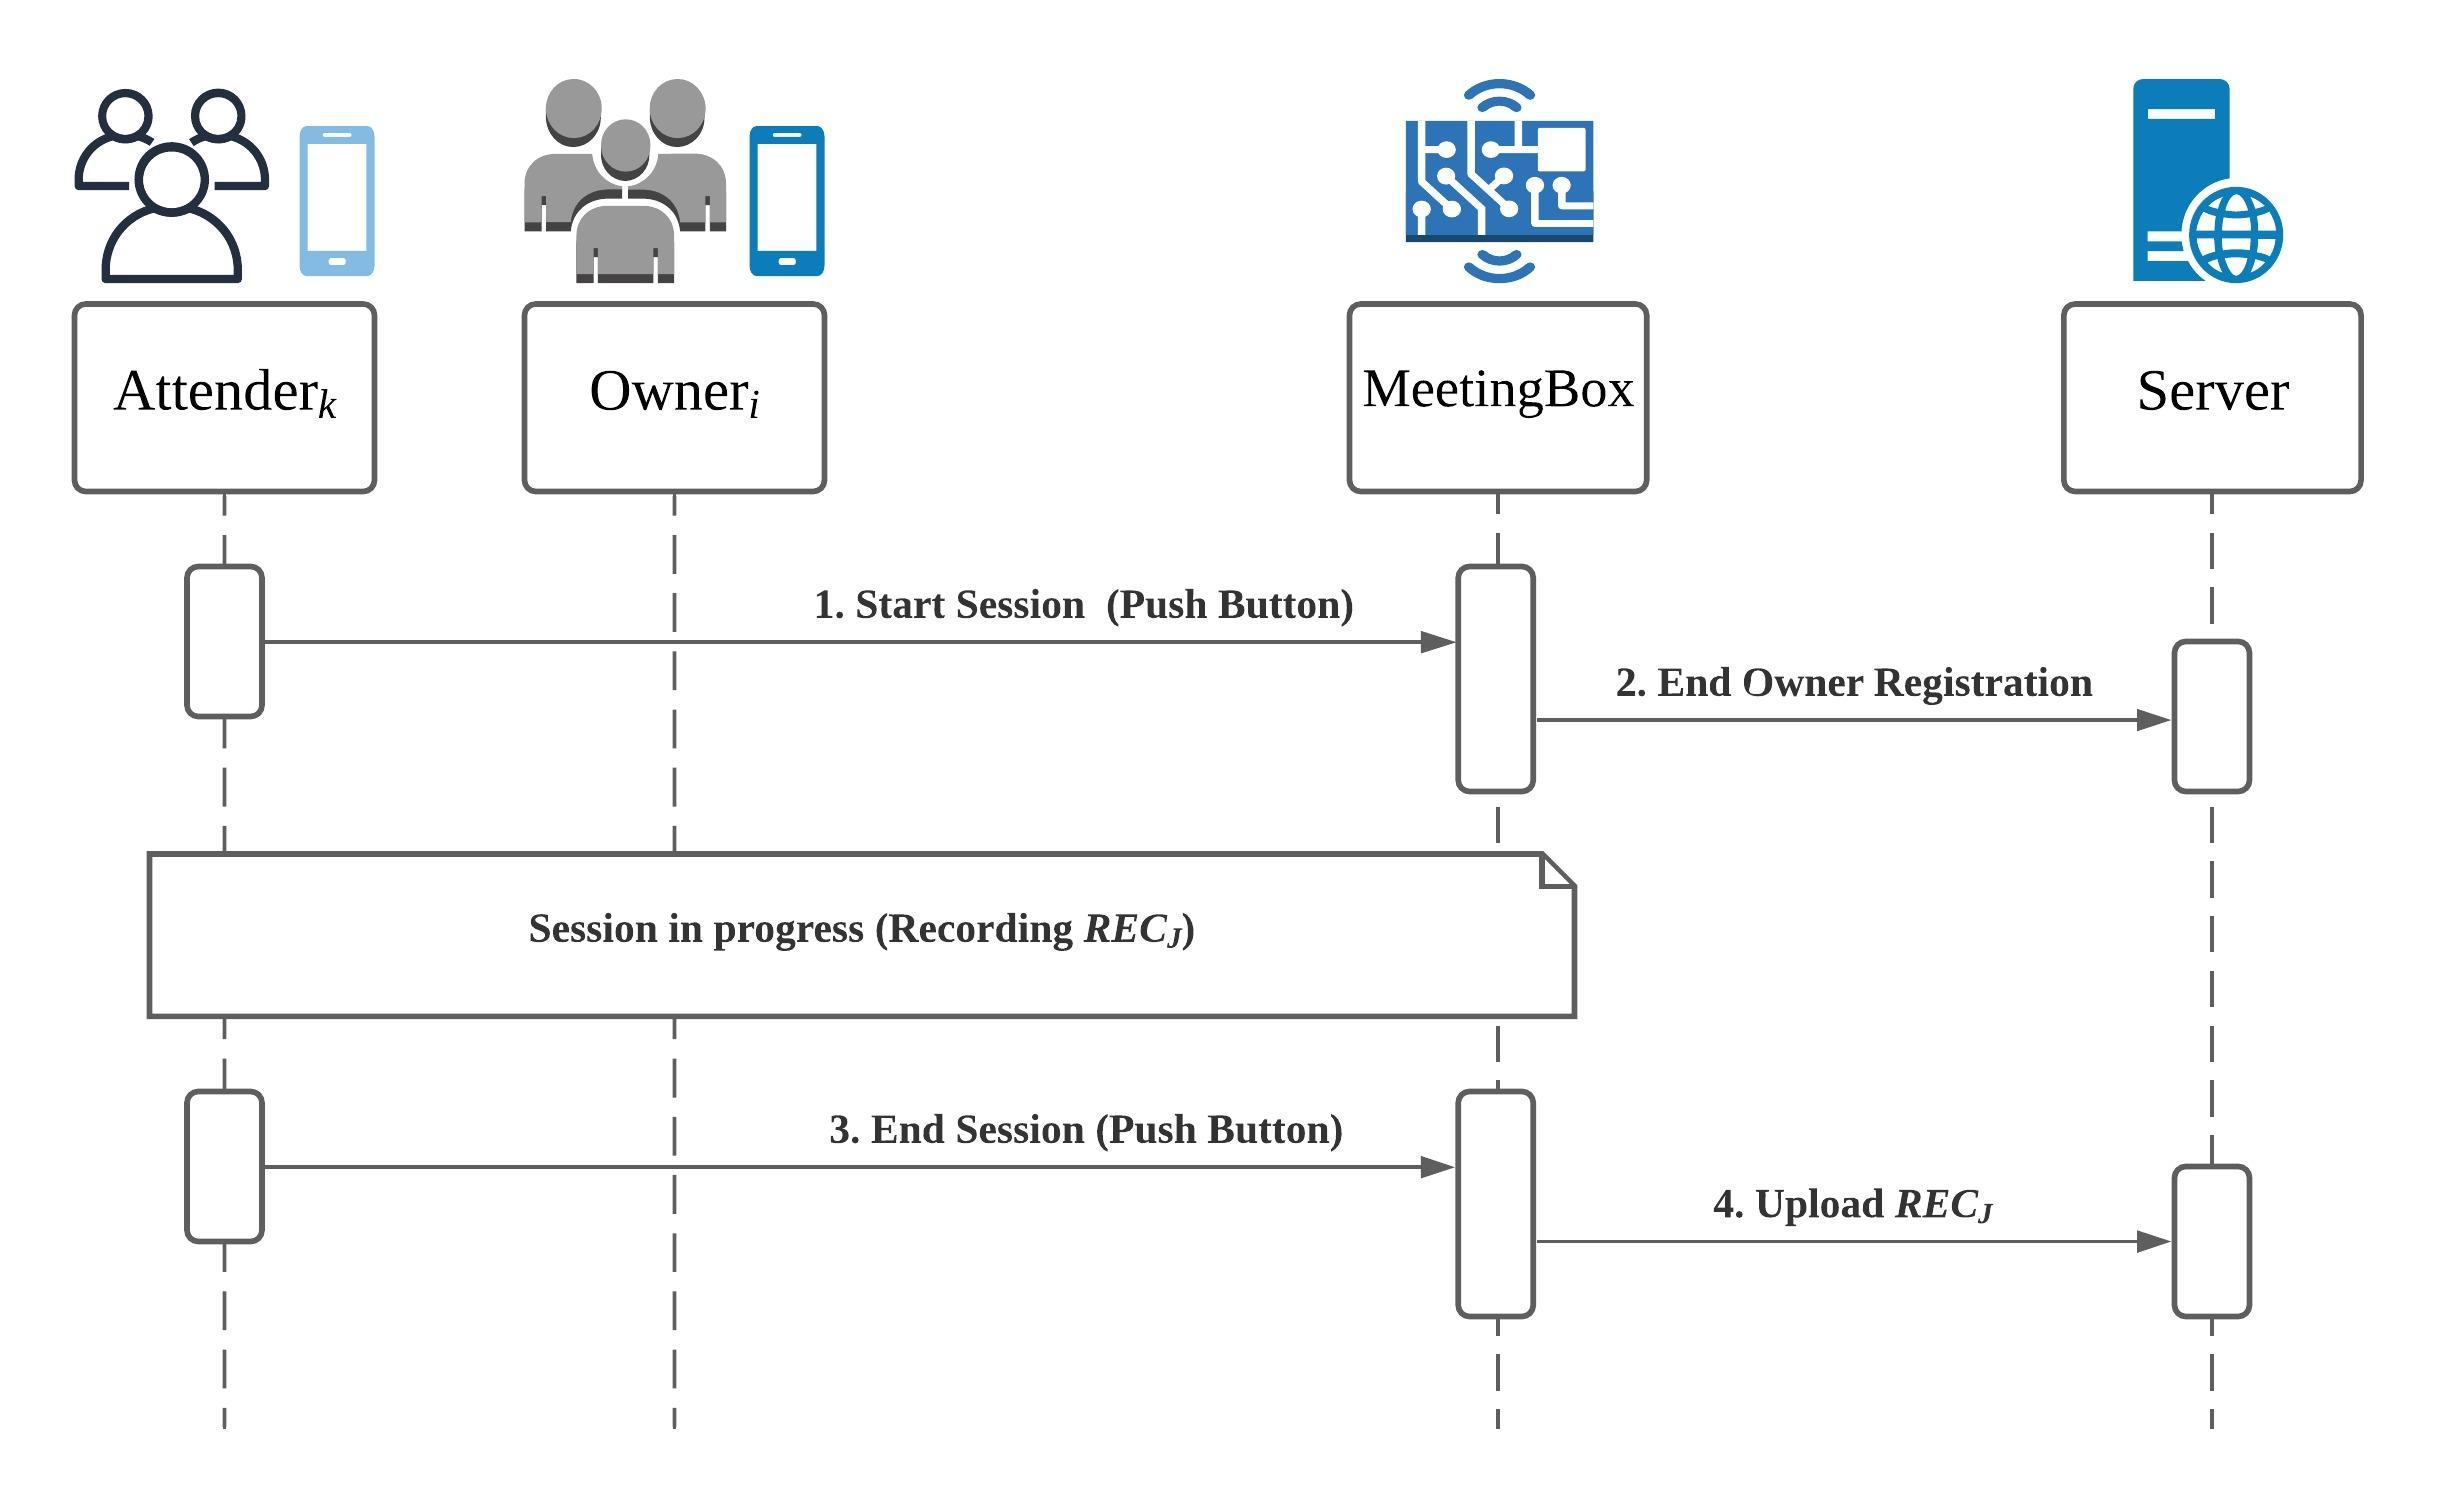
\includegraphics[width=0.8\textwidth]{multi-owner-sequence-diagram-sessioning}
    \caption{進行會談於多會談主持者情境}\label{fig:m-o-sessioning}
\end{figure}

    圖中步驟 1\textasciitilde4 與
 \ref{subsec:sessioning} \nameref{fig:s-o-sessioning} 中的流程步驟相同。

    於多會談主持者 ({\it Multi Owner}) 情境中,
會談生命週期第三個階段「解封會談聲音記錄」(Unsealing Session Record)」的系統流程。
如圖 \ref{fig:m-o-unseal} 所示。

\begin{figure}[H]
    \centering
    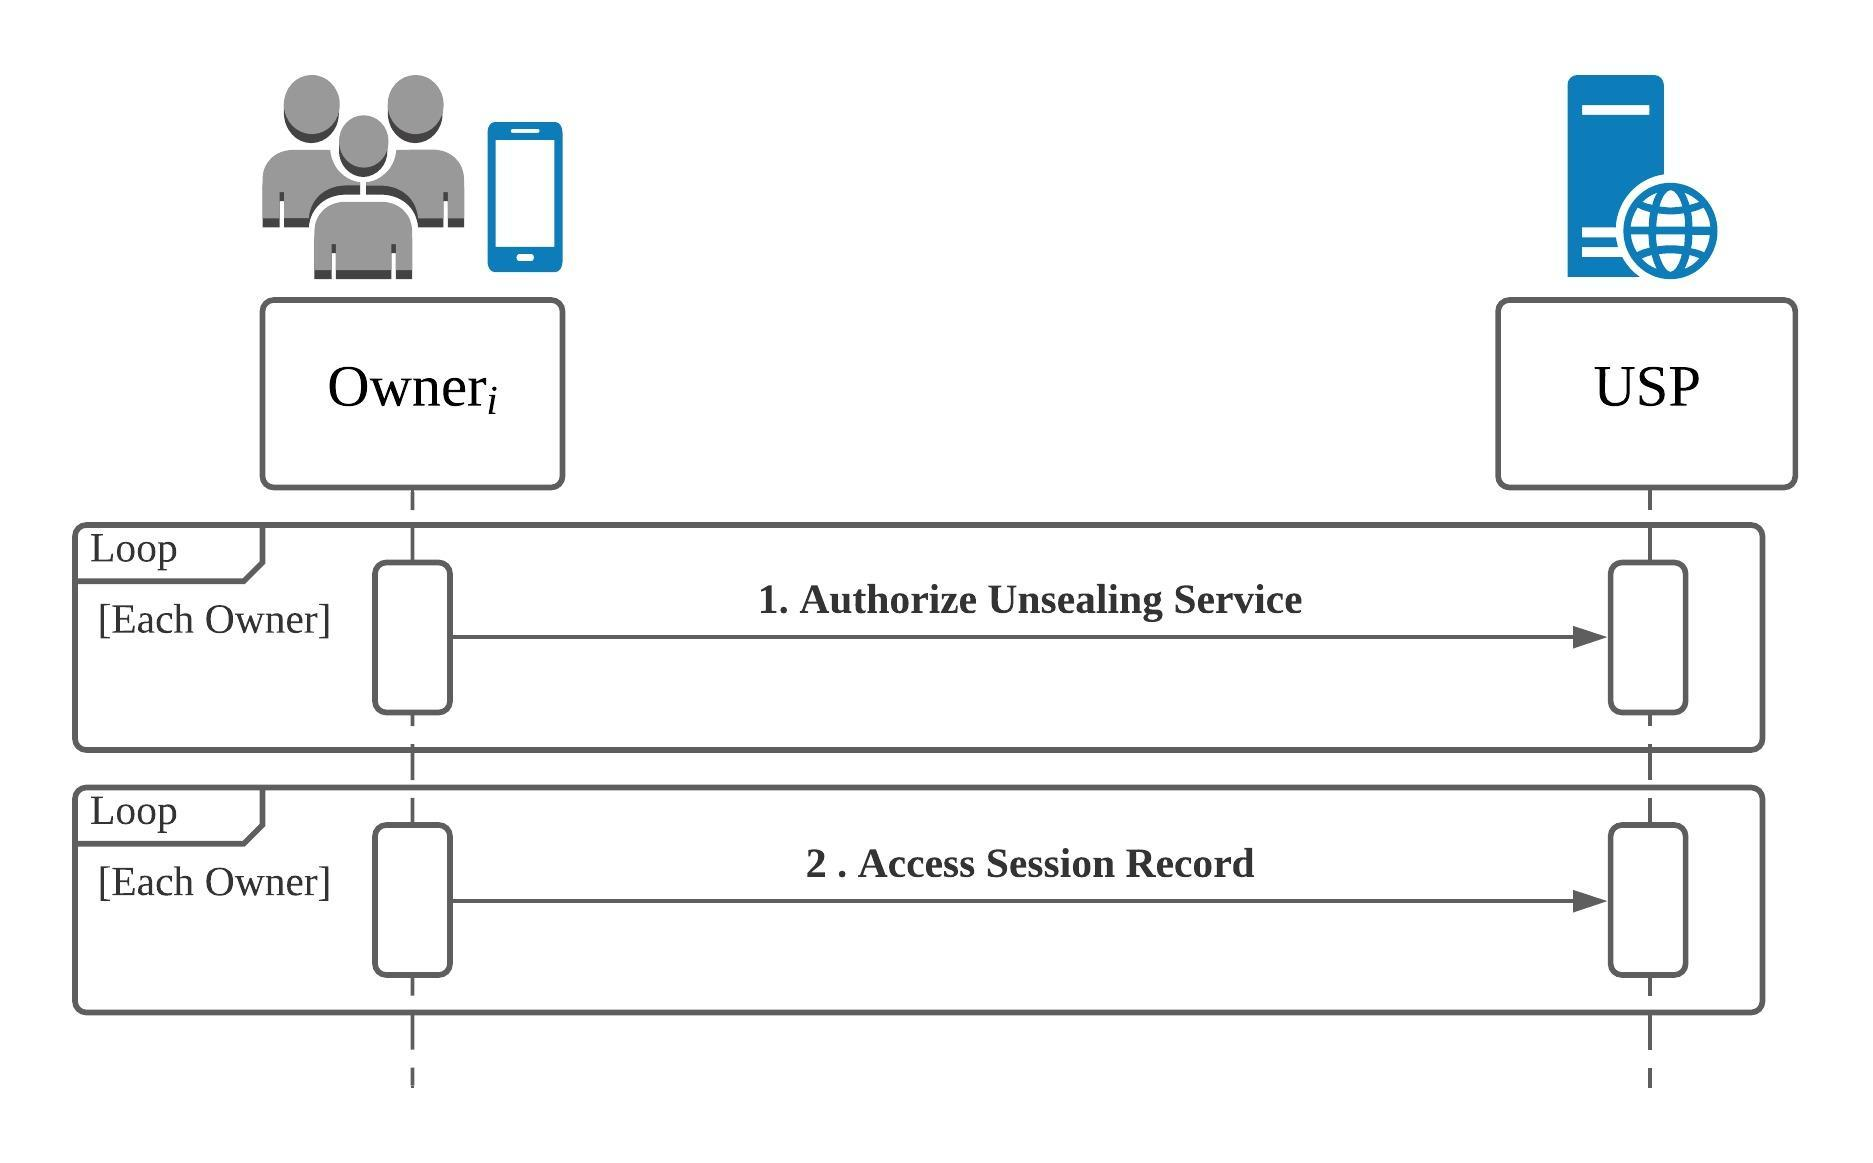
\includegraphics[width=0.7\textwidth]{multi-owner-sequence-diagram-unseal}
    \caption{解封會談聲音記錄於多會談主持者情境}\label{fig:m-o-unseal}
\end{figure}

    圖中步驟 1\textasciitilde2 與 3\textasciitilde4
分別與 \ref{subsec:unseal} \nameref{fig:s-o-unseal} 中的流程步驟相同。

    其中步驟 1\textasciitilde2 需要所有的會談主持者 \DEFownerAll 執行,
各會談主持者 \DEFowner 可以同時獨立執行,待每位會談主持者 \DEFowner 執行成功後,即完成授權。
若有任何一位會談主持者 \DEFowner 執行失敗,即授權失敗。

    最後步驟 3\textasciitilde4 為各會談主持者 \DEFowner 自行選擇執行與否,以取得此有效之會談聲音記錄。


\section{聲音記錄存取控制協定}\label{sec:protocol}

    本節基於前章節 \ref{sec:system-flow} \nameref{sec:system-flow},延伸出一套聲音記錄存取控制協定。
其中包括創建會談、註冊會談主持者、進行會談、會談主持者授權解封伺服器、取得會談聲音記錄。

    會談終端 \DEFmeetingbox 於談生命週期開始之前,
會預先設定時間長度為 \DEFtimeMAX 的純噪音之聲音記錄 \DEFrecN,
受干擾的會談聲音記錄 \DEFrecJ 之內容長度,須小於 \DEFtimeMAX。
此純噪音之聲音記錄 \DEFrecN 為純超音波麥克風干擾器於麥克風的響應輸出之聲音記錄,
產生方法為選定一隨機種子 \DEFseed 作為參數,輸入並開啟超音波麥克風干擾器,透過麥克風錄製產生。
每次選定的隨機種子 \DEFseed 皆不同,因此每次配置產生 \DEFrecN 也不同。
於每次會談生命週期結束後,重複執行此步驟重新選定隨機種子 \DEFseed 與產生純噪音之聲音記錄 \DEFrecN。


\subsection{創建會談階段}\label{subsec:protocol-init-create}

    在會談生命週期的\nameref{subsec:initialize}中,
當會談參與者透過與會談終端的物理控制介面執行建立會談(圖 \ref{fig:m-o-init}步驟 1),
會談終端獲得外部事件而觸發執行此階段。

    每次會談生命週期結束後,會談終端 \DEFmeetingbox 皆會為未來新的會談生命週期重新配置產生
純超音波麥克風干擾器於麥克風的響應輸出(純噪音)之聲音記錄 \DEFrecN,
此時會談終端 \DEFmeetingbox 應存在純噪音之聲音記錄 \DEFrecN。

    此階段為\ref{subsec:initialize} \nameref{subsec:initialize}中的步驟 2\textasciitilde3,
其運作細節如圖 \ref{fig:protocol-init-create}與說明:

\begin{center}\scriptsize\setstretch{1}
\begin{tabularx}{0.8\textwidth} {
        |c
        >{\raggedright\arraybackslash}X
        >{\centering\arraybackslash}c
        >{\raggedright\arraybackslash}X
        c|
    }
    \hline

    \multicolumn{5}{|c|}{} \\
    & \multicolumn{1}{c}{\small{\DEFmeetingbox}} &
    & \multicolumn{1}{c}{\small{\DEFserver}} & \\
    %
    & \multicolumn{1}{c}{$\{$\DEFrecN$\}$} &
    & \multicolumn{1}{c}{} & \\
    %
    \cline{2-2} \cline{4-4}
    \multicolumn{5}{|c|}{} \\

    &
    $M_{1}$ $\leftarrow$ $\{\}$
    & & & \\

    & &
    $\xrightarrow{ \qquad M_{1} \qquad }$
    & & \\

    & & &
    \DEFsessionID $\leftarrow$ \DEFfuncIDgen{} \newline
    \DEFunsealKey $\leftarrow$ \DEFfuncKgen{} \newline
    \DEFowreg $\leftarrow$ $0$ \newline
    {\bf bind relations:} \newline
    \pcind \DEFunsealKey ~ $\in$ ~ \DEFsessionID \newline
    $M_{2}$ $\leftarrow$ $\{$\DEFsessionID, \DEFunsealKey$\}$
    & \\

    & &
    $\xleftarrow{ \qquad M_{2} \qquad }$
    & & \\

    &
    $k$ $\leftarrow$ \DEFunsealKey \newline
    $m_{3}$ $\leftarrow$ \DEFfuncEncEK{\DEFrecN} \newline
    $M_{3}$ $\leftarrow$ $\{$\DEFsessionID, $m_{3}$$\}$ \newline
    & & & \\

    & &
    $\xrightarrow{ \qquad M_{3} \qquad }$
    & & \\

    & & &
    \DEFrecP $\leftarrow$ $m_{3}$ \newline
    {\bf bind relations:} \newline
    \pcind \DEFrecP ~ $\in$ ~ \DEFsessionID \newline
    $M_{4}$ $\leftarrow$ $\{\}$
    & \\

    & &
    $\xleftarrow{ \qquad M_{4} \qquad }$
    & & \\

    &
    {\bf destroy~} \DEFunsealKey
    & & & \\

    \multicolumn{5}{|c|}{} \\
    \hline
\end{tabularx}
\captionsetup{hypcap=false}
\captionof{figure}{創建會談階段}\label{fig:protocol-init-create}
\setstretch{1.2}\normalsize\end{center}

\begin{pmsgs}
    \item $\{\}$ $,~$ \DEFmeetingbox $\rightarrow$ \DEFserver:

        當會談終端 \DEFmeetingbox 獲得外部事件,
    觸發會談終端向解封伺服器 \DEFserver 發送請求創建新的會談。

    \item $\{$\DEFsessionID, \DEFunsealKey$\}$ $,~$ \DEFserver $\rightarrow$ \DEFmeetingbox:

        解封伺服器 \DEFserver 收到請求後,執行 \DEFfuncIDgen{} 與 \DEFfuncKgen{},
    分別產生此次會談的唯一識別碼 \DEFsessionID,與此次會談的解封金鑰 \DEFunsealKey。
    首先將 \DEFunsealKey 關聯綁定屬於 \DEFsessionID。接著建立變數 \DEFowreg,
    定義為此會談的會談主持者於解封伺服器 \DEFserver 的註冊人數,初始值為 $0$。
    隨後回覆會談終端 \DEFmeetingbox,會談創建成功,訊息內容為 \DEFsessionID 與 \DEFunsealKey。

        其中 \DEFfuncIDgen{} 為唯一識別碼產生函數,其產生須滿足唯一性、隨機性、不可預測性。
    \DEFfuncKgen{} 為對稱式加密演算法的金鑰產生函數。\DEFunsealKey 為對稱式加密金鑰。

    \item $\{$\DEFsessionID, \DEFrecP$\}$ $,~$ \DEFmeetingbox $\rightarrow$ \DEFserver:

        會談終端 \DEFmeetingbox 收到來自 \DEFserver 的回覆後,
    使用 \DEFunsealKey 透過對稱式加密函數 \DEFfuncEncEK{}
    加密預先配置好的純超音波麥克風干擾器之聲音記錄(噪音) \DEFrecN,定義為 \DEFrecP,
    接著向解封伺服器發出上傳請求,
    訊息內容為此次會談的唯一識別碼 \DEFsessionID 與受加密保護的聲音記錄 \DEFrecP。

    \item $\{\}$ $,~$ \DEFserver $\rightarrow$ \DEFmeetingbox:

        解封伺服器 \DEFserver 收到訊息後,將 \DEFrecP 關聯綁定屬於 \DEFsessionID。
    隨後回覆會談終端 \DEFmeetingbox 上傳成功。
    會談終端 \DEFmeetingbox 收到來自解封伺服器 \DEFserver 的上傳成功回覆後,
    銷毀於會談終端上的 \DEFrecN 與 \DEFunsealKey。
\end{pmsgs}


\subsection{註冊會談主持者階段}\label{subsec:protocol-init-reg}

    於會談生命週期同一階段\nameref{subsec:initialize}中,
當談終端 \DEFmeetingbox 獲得產自解封伺服器的元資料後,
會談終端上的人機互動介面提示予所有會談主持者 \DEFownerAll,
可以執行本協定之 \nameref{fig:protocol-init-reg}。

    在此階段中,會談已執行完成前篇\nameref{subsec:protocol-init-create}。
此時會談終端 \DEFmeetingbox 應已獲得此次會談唯一識別碼 \DEFsessionID。
解封伺服器 \DEFserver 中也應存在資料包含會談主持者註冊人數 \DEFowreg 及此次會談唯一識別碼 \DEFsessionID。

    此階段需要所有的會談主持者 \DEFownerAll 執行,各會談主持者 \DEFowner 可以同時獨立執行,
每個會談主持者 \DEFowner 的執行結果不受其他會談主持者影響。

    此階段為 \ref{subsec:initialize} \nameref{subsec:initialize}中的步驟 4\textasciitilde5,
其運作細節如圖 \ref{fig:protocol-init-reg}與說明:

\begin{center}\scriptsize\setstretch{1}
\begin{tabularx}{0.95\textwidth} {
        |c
        >{\raggedright\arraybackslash}X
        >{\centering\arraybackslash}c
        >{\raggedright\arraybackslash}X
        >{\centering\arraybackslash}c
        >{\raggedright\arraybackslash}X
        c|
    }
    \hline

    \multicolumn{7}{|c|}{} \\
    & \multicolumn{1}{c}{\small{\DEFowner}} &
    & \multicolumn{1}{c}{\small{\DEFmeetingbox}} &
    & \multicolumn{1}{c}{\small{\DEFserver}} & \\
    %
    & \multicolumn{1}{c}{} &
    & \multicolumn{1}{c}{$\{$\DEFsessionID$\}$} &
    & \multicolumn{1}{c}{$\{$\DEFsessionID, \DEFowreg$\}$} & \\
    %
    \cline{2-2} \cline{4-4} \cline{6-6}
    \multicolumn{7}{|c|}{} \\

    & {\bf for each~} \DEFowner $\in$ \DEFownerAll \newline
    \pcind {\bf where~} $i=1~...\mid$\DEFownerAll$\mid$ {\bf:}
    & & & & & \\

    \cdashline{2-6}

    \rule{0pt}{10pt} & \multicolumn{1}{:l}{
    \pcind\pcind $M_{1}^{i}$ $\leftarrow$ $\{\}$
    } & & & & \multicolumn{1}{l:}{} & \\

    & \multicolumn{1}{:l}{} &
    $\xrightarrow{ \enskip M_{1}^{i} \enskip }$
    & & & \multicolumn{1}{l:}{} & \\

    & \multicolumn{1}{:l}{} & &
    $M_{2}^{i}$ $\leftarrow$ $\{$\DEFsessionID$\}$
    & $\quad\quad\quad\quad$ & \multicolumn{1}{l:}{} & \\

    & \multicolumn{1}{:l}{} &
    $\xleftarrow{ \enskip M_{2}^{i} \enskip }$
    & & & \multicolumn{1}{l:}{} & \\

    & \multicolumn{1}{:l}{
    \pcind\pcind $M_{3}^{i}$ $\leftarrow$ $\{$\DEFsessionID$\}$
    } & & & & \multicolumn{1}{l:}{} & \\

    & \multicolumn{1}{:l}{} & \multicolumn{3}{c}{
    $\xrightarrow{\qquad\qquad\qquad\qquad\qquad M_{3}^{i} \qquad\qquad\qquad\qquad\qquad}$
    }& \multicolumn{1}{l:}{} & \\

    & \multicolumn{1}{:l}{} & & & & \multicolumn{1}{l:}{\shortstack[l]{
    $($\DEFpublicKey, \DEFprivateKey$)$ $\leftarrow$ \DEFfuncPKgen{} \\
    \DEFownerID $\leftarrow$ \DEFfuncIDgen{}{} \\
    {\bf bind relations:} \\
    \pcind \DEFownerID $\in$ \DEFsessionID \\
    \pcind \DEFpublicKey $\in$ \DEFownerID \\
    \DEFowreg $\leftarrow$ \DEFowreg $+1$ \\
    $M_{4}^{i}$ $\leftarrow$ $\{$\DEFownerID, \DEFprivateKey$\}$
    }} & \\

    & \multicolumn{1}{:l}{} & \multicolumn{3}{c}{
    $\xleftarrow{\qquad\qquad\qquad\qquad\qquad M_{4}^{i} \qquad\qquad\qquad\qquad\qquad}$
    }& \multicolumn{1}{l:}{} & \\

    & \multicolumn{1}{:l}{
    \pcind\pcind {\bf store~} $\{$\DEFownerID, \DEFprivateKey$\}$
    } & & & & \multicolumn{1}{l:}{
    {\bf destroy~} \DEFprivateKey
    } & \\

    & \multicolumn{1}{:l}{} & & & & \multicolumn{1}{l:}{} & \\
    \cdashline{2-6}

    \multicolumn{7}{|c|}{} \\
    \hline
\end{tabularx}
\captionsetup{hypcap=false}
\captionof{figure}{註冊會談主持者階段}\label{fig:protocol-init-reg}
\setstretch{1.2}\normalsize\end{center}

\begin{pmsgsi}
    \item $\{\}$ $,~$ \DEFowner $\rightarrow$ \DEFmeetingbox:

        當會談主持者 \DEFowner 觀察到於會談終端 \DEFmeetingbox 上的人機互動介面提示,
    向發會談終端送請求獲得會談的元資料。

    \item $\{$\DEFsessionID$\}$ $,~$ \DEFmeetingbox $\rightarrow$ \DEFowner:

        會談終端 \DEFmeetingbox 收到請求後,回覆此次會談的元資料給會談主持者 \DEFowner,
    訊息內容為此次會談的唯一識別碼 \DEFsessionID。

    \item $\{$\DEFsessionID$\}$ $,~$ \DEFowner $\rightarrow$ \DEFserver:

        會談主持者 \DEFowner 獲得此次會談的元資料後,便可向解封伺服器 \DEFserver 傳送註冊請求,
    訊息內容為此次會談的唯一識別碼 \DEFsessionID。

    \item $\{$\DEFownerID, \DEFprivateKey$\}$ $,~$ \DEFserver $\rightarrow$ \DEFowner:

        解封伺服器 \DEFserver 收到註冊請求後,執行 \DEFfuncPKgen{} 與 \DEFfuncIDgen{},
    分別產生一組屬於會談主持者 \DEFowner 的公開私密金鑰對 $($\DEFpublicKey$,~$ \DEFprivateKey$)$,
    與此會談主持者 \DEFowner 的唯一識別碼 \DEFownerID。

        會談主持者的唯一識別碼 \DEFownerID,其產生須滿足唯一性、隨機性、不可預測性。
    \DEFfuncPKgen{} 為非對稱加密演算法的公開私密金鑰對產生函數。

        接著將此次會談的會談主持者註冊人數 \DEFowreg 遞增 $1$,
    並將 \DEFownerID 關聯綁定屬於 \DEFsessionID,\DEFpublicKey 關聯綁定屬於 \DEFownerID 並儲存。
    隨後回傳 \DEFownerID 與其私鑰 \DEFprivateKey,並銷毀 \DEFprivateKey。

        會談主持者收到解封伺服器 \DEFserver 的回傳即註冊成功。
    會談主持者為會談參與者中的特權角色,其特權來源為會傳訊息內的 \DEFprivateKey,
    因此會談主持者須妥善保管 \DEFprivateKey,維持其機密性。
    待所有的會談主持者 \DEFownerAll 執行成功此階段後,即完成會談生命週期中的初始化會談。
\end{pmsgsi}


\subsection{進行會談階段}\label{subsec:protocol-sessioning}

    在會談生命週期的\nameref{subsec:sessioning}中,
會談參與者透過與會談終端的物理控制介面(圖 \ref{fig:m-o-sessioning} 步驟 1、3),
使會談終端獲得外部事件而發執行此階段。

    在此階段中,會談已完成會談生命週期第一階段\nameref{subsec:initialize}。
此時會談終端應已獲得此次會談唯一識別碼 \DEFsessionID。
解封伺服器 \DEFserver 中也應存在資料包含會談主持者註冊人數 \DEFowreg、
屬於此次會談唯一識別碼的所有會談主持者唯一識別碼 \DEFownerID 與其 \DEFpublicKey。

    此階段為 \ref{subsec:sessioning} \nameref{subsec:sessioning}中的步驟 4\textasciitilde5,
完成後系統將產生被干擾的會談聲音記錄 \DEFrecJ 與受加密保護的授權金鑰 \DEFakEnc。
其運作細節如圖 \ref{fig:protocol-sessioning}與說明:

\begin{center}\scriptsize\setstretch{1}
\begin{tabularx}{0.95\textwidth} {
        |c
        >{\raggedright\arraybackslash}X
        >{\centering\arraybackslash}c
        >{\raggedright\arraybackslash}X
        c|
    }
    \hline

    \multicolumn{5}{|c|}{} \\
    & \multicolumn{1}{c}{\small{\DEFmeetingbox}} &
    & \multicolumn{1}{c}{\small{\DEFserver}} & \\
    %
    & \multicolumn{1}{c}{$\{$\DEFsessionID, \DEFrecJ$\}$} &
    & \multicolumn{1}{c}{$\{$
        \DEFsessionID,
        \DEFowreg,
        $\{[($ \DEFownerID, \DEFpublicKey $)] \mid i=1~...$\DEFowreg $\}\}$}
    & \\
    %
    \cline{2-2} \cline{4-4}
    \multicolumn{5}{|c|}{} \\

    &
    $M_{1}$ $\leftarrow$ $\{$\DEFsessionID$\}$
    & & & \\

    & &
    $\xrightarrow{ \enskip M_{1} \enskip }$
    & & \\

    & & &
    {\bf if~} \DEFowreg $=1${\bf:} \newline
    \pcind $pk$ $\leftarrow$ \DEFpublicKey \newline
    \pcind \DEFakEnc $\leftarrow$ \DEFfuncEncPK{\DEFunsealKey} \newline
    \pcind {\bf bind relations:} \newline
    \pcind\pcind \DEFakEnc $\in$ \DEFownerID \newline

    {\bf if~} \DEFowreg $>1${\bf:} \newline
    \pcind $c$ $\leftarrow$ \DEFowreg \newline
    \pcind $t$ $\leftarrow$ \DEFowreg \newline
    \pcind $[s_{i}]$ $\leftarrow$ \DEFfuncSSS{\DEFunsealKey} \newline
    \pcind {\bf for each~} $s_{i} \in [s_{i}]$~ {\bf where~} $i=1~...$\DEFowreg {\bf:} \newline
    \pcind\pcind $pk$ $\leftarrow$ \DEFpublicKey \newline
    \pcind\pcind \DEFakEnc $\leftarrow$ \DEFfuncEncPK{$s_{i}$} \newline
    \pcind\pcind {\bf destroy~} $s_{i}$ \newline
    \pcind\pcind {\bf bind relations:} \newline
    \pcind\pcind\pcind \DEFakEnc $\in$ \DEFownerID \newline

    {\bf destroy~} \DEFunsealKey \newline
    $M_{2}$ $\leftarrow$ $\{\}$
    & \\

    & &
    $\xleftarrow{ \enskip M_{2} \enskip }$
    & & \\

    \multicolumn{5}{|c|}{} \\
    \cline{2-2}
    & \multicolumn{1}{|c|}{} & & & \\
    & \multicolumn{1}{|c|}{Session in progress (Recording \DEFrecJ)} & & & \\
    & \multicolumn{1}{|c|}{} & & & \\
    \cline{2-2}
    \multicolumn{5}{|c|}{} \\

    &
    $M_{3}$ $\leftarrow$ $\{$\DEFsessionID, \DEFrecJ$\}$
    & & & \\

    & &
    $\xrightarrow{ \enskip M_{3} \enskip }$
    & & \\

    & & &
    {\bf bind relations:} \newline
    \pcind \DEFrecJ ~ $\in$ ~ \DEFsessionID \newline
    $M_{4}$ $\leftarrow$ $\{\}$
    & \\

    & &
    $\xleftarrow{ \enskip M_{4} \enskip }$
    & & \\

    \multicolumn{5}{|c|}{} \\
    \hline
\end{tabularx}
\captionsetup{hypcap=false}
\captionof{figure}{進行會談階段}\label{fig:protocol-sessioning}
\setstretch{1.2}\normalsize\end{center}

\begin{pmsgs}
    \item $\{$\DEFsessionID$\}$ $,~$ \DEFmeetingbox $\rightarrow$ \DEFserver:

        會談參與者透過與會談終端的物理控制介面,
    使會談終端 \DEFmeetingbox 獲得外部事件而觸發向解封伺服器 \DEFserver 發出此請求,
    目標為通知解封伺服器 \DEFserver,會談主持者註冊已完成。
    訊息內容為此次會談唯一識別碼 \DEFsessionID。

    \item $\{\}$ $,~$ \DEFserver $\rightarrow$ \DEFmeetingbox:

        解封伺服器收到會談終端的請求後,
    透過限制會談唯一識別 \DEFsessionID 不再新增關聯綁定新的會談主持者,來終止會談主持者註冊。
    接著判斷會談主持者註冊人數 \DEFowreg 是否為一或多人。

        若為一人,則為單一會談主持者情境。此時將屬於此會談的解封金鑰 \DEFunsealKey,
    透過唯一會談主持者 \DEFowner 的非對稱式公開金鑰 \DEFpublicKey,
    使用非對稱式金鑰演算法加密函數 \DEFfuncEncPK{} 加密。因僅有單一會談主持者,
    加密後的解封金鑰 \DEFunsealKey,則視為唯一會談主持者 \DEFowner 的受加密保護的授權金鑰 \DEFakEnc。

        若為多人,則為多會談主持者情境。此時將屬於此會談的解封金鑰 \DEFunsealKey,
    透過金鑰分割函數 \DEFfuncSSS{},根據會談主持者註冊人數 \DEFowreg,
    分割成 \DEFowreg 份分割秘密 \DEFsharesAll。
    再將每個分割秘密 \DEFshares,透過每個會談主持者 \DEFowner 的公開金鑰 \DEFpublicKey,
    使用非對稱式金鑰演算法加密函數 \DEFfuncEncPK{} 加密,並銷毀該分割秘密。
    受加密保護的分割秘密,即定義為該會談主持者 \DEFowner 的受加密保護的授權金鑰 \DEFakEnc。

        當所有會談主持者 \DEFowner 的受加密保護的授權金鑰 \DEFakEnc 產生完畢。
    隨即銷毀該會談的解封金鑰 \DEFunsealKey,並回覆註冊終止成功。

        會談終端 \DEFmeetingbox 收到解封伺服器的回覆後,終止註冊完成。
    此時開啟會談終端上的超音波麥克風干擾器與麥克風,並於人機互動介面提示系統已開始錄音,
    開始紀錄受干擾的會談聲音 \DEFrecJ。此為超音波麥克風干擾器與會談聲音內容的疊加,屬非有效之聲音記錄。
    此時會談參與者 \DEFattenderAll 即可進行私密會談,不用擔心存在其他麥克風或聲音記錄裝置可以取得有效之聲音記錄。

    \item $\{$\DEFsessionID, \DEFrecJ$\}$ $,~$ \DEFmeetingbox $\rightarrow$ \DEFserver:

        當會談參與者再次透過與會談終端的物理控制介面,
    使會談終端 \DEFmeetingbox 獲得外部事件,此時觸發會談聲音記錄終止,關閉麥克風與超音波麥克風干擾器,
    受干擾的會談聲音紀錄 \DEFrecJ 錄製完成。並於人機互動介面提示系統已結束錄音。
    接著會談終端 \DEFmeetingbox 向解封伺服器 \DEFserver 發出上傳請求,
    內容為此次會談唯一識別碼 \DEFsessionID 與受干擾的會談聲音紀錄 \DEFrecJ。

    \item $\{\}$ $,~$ \DEFserver $\rightarrow$ \DEFmeetingbox:

        解封伺服器收到會談終端的請求後,
    將受干擾的會談聲音紀錄 \DEFrecJ 關聯綁定屬於 \DEFsessionID 且儲存,隨後回覆上傳成功。
    此時會談參與者即可離開會談場域,不再需要與會談終端 \DEFmeetingbox 實體接觸。

        隨後會談終端開始為未來新的會談生命週期重新配置產生新 \DEFrecN,
    產生方法為選定一隨機種子 \DEFseed 作為參數,輸入並開啟超音波麥克風干擾器,透過麥克風錄製產生。
    每次選定的隨機種子 \DEFseed 皆不同,因此每次配置產生 \DEFrecN 也不同。
\end{pmsgs}


\subsection{會談主持者授權解封伺服器階段}\label{subsec:protocol-unseal-auth}

    本章描述之協定為會談生命週期中的\nameref{subsec:unseal}階段(圖 \ref{fig:m-o-unseal})中的步驟 1,
當會談主持者 \DEFowner 欲取得當時會談的聲音記錄,則執行此階段。
目標為使會談主持者 \DEFowner 授權解封伺服器 \DEFserver,使其有權限可以執行後續階段。

    在此階段中,會談主持者 \DEFowner 已完成前篇\nameref{subsec:protocol-init-reg}。
此時會談主持者 \DEFowner 持有包含此次會談唯一識別碼 \DEFsessionID、會談主持者唯一識別碼 \DEFownerID
與會談主持者私密金鑰 \DEFprivateKey。
解封伺服器 \DEFserver 也應儲存有包含此次會談唯一識別碼 \DEFsessionID、會談主持者註冊人數 \DEFowreg、
所有會談主持者的唯一識別碼 \DEFownerID、屬於此會談主持者的公開金鑰 \DEFprivateKey
與屬於各會談主持者的受加密保護的授權金鑰 \DEFakEnc。

    此階段需要所有的會談主持者 \DEFownerAll 執行,各會談主持者 \DEFowner 可以同時獨立執行,
每位會談主持者 \DEFowner 的執行成功後,即完成授權。

    此階段為 \ref{subsec:unseal} \nameref{subsec:unseal}中的步驟 1,
其運作細節如圖 \ref{fig:protocol-unseal-auth}與說明:

\begin{center}\scriptsize\setstretch{1}
\begin{tabularx}{0.95\textwidth} {
        |c
        >{\raggedright\arraybackslash}X
        >{\centering\arraybackslash}c
        >{\raggedright\arraybackslash}X
        c|
    }
    \hline

    \multicolumn{5}{|c|}{} \\
    & \multicolumn{1}{c}{\small{\DEFowner}} &
    & \multicolumn{1}{c}{\small{\DEFserver}} & \\
    %
    & \multicolumn{1}{c}{$\{$ \DEFsessionID,
        $\{[($ \DEFownerID, \DEFprivateKey $)] \mid i=1~...\mid$\DEFownerAll$\mid$ $\}\}$}
    & & \multicolumn{1}{c}{\shortstack[c]{$\{$
        \DEFsessionID,
        $\{[($ \DEFownerID, \DEFpublicKey, \DEFakEnc $)] \mid i=1~...$\DEFowreg $\}\}$}}
    & \\
    %
    \cline{2-2} \cline{4-4}
    \multicolumn{5}{|c|}{} \\

    & {\bf for each~} \DEFowner $\in$ \DEFownerAll \newline
    \pcind {\bf where~} $i=1~...\mid$\DEFownerAll$\mid$ {\bf:}
    & & & \\

    \cdashline{2-4}

    \rule{0pt}{10pt} & \multicolumn{1}{:l}{
    \pcind\pcind $M_{1}^{i}$ $\leftarrow$ $\{$\DEFsessionID, \DEFownerID$\}$
    } & & \multicolumn{1}{l:}{} & \\

    & \multicolumn{1}{:l}{} &
    $\xrightarrow{ \enskip M_{1}^{i} \enskip }$
    & \multicolumn{1}{l:}{} & \\

    & \multicolumn{1}{:l}{} & & \multicolumn{1}{l:}{
    $M_{2}^{i}$ $\leftarrow$ $\{$\DEFownerID, \DEFakEnc$\}$
    } & \\

    & \multicolumn{1}{:l}{} &
    $\xleftarrow{ \enskip M_{2}^{i} \enskip }$
    & \multicolumn{1}{l:}{} & \\

    & \multicolumn{1}{:l}{\shortstack[l]{
    \pcind\pcind $sk$ $\leftarrow$ \DEFprivateKey \\
    \pcind\pcind $m_{3}$ $\leftarrow$ \DEFfuncDecSK{\DEFakEnc} \\
    \pcind\pcind $m_{3}.sig$ $\leftarrow$ \DEFfuncSignSK{$m_{3}$} \\
    \pcind\pcind $M_{3}^{i}$ $\leftarrow$ $\{$\DEFownerID$, m_{3}, ~m_{3}.sig\}$
    }} & & \multicolumn{1}{l:}{} & \\

    & \multicolumn{1}{:l}{} &
    $\xrightarrow{ \enskip M_{3}^{i} \enskip }$
    & \multicolumn{1}{l:}{} & \\

    & \multicolumn{1}{:l}{} & & \multicolumn{1}{l:}{\shortstack[l]{
    $pk$ $\leftarrow$ \DEFpublicKey \\
    $valid$ $\leftarrow$ \DEFfuncVerfPK{$m_{3},~m_{3}.sig$} \\
    {\bf if} !$valid$ {\bf :} \\
    \pcind {\bf terminate session} \\
    {\bf else} {\bf :} \\
    \pcind \DEFagentKey $\leftarrow$ $m_{3}$ \\
    \pcind {\bf bind relations:} \\
    \pcind\pcind \DEFagentKey $\in$ \DEFownerID \\
    $M_{4}^{i}$ $\leftarrow$ $\{\}$
    }} & \\

    & \multicolumn{1}{:l}{} &
    $\xleftarrow{ \enskip M_{4}^{i} \enskip }$
    & \multicolumn{1}{l:}{} & \\

    & \multicolumn{1}{:l}{} & & \multicolumn{1}{l:}{} & \\
    \cdashline{2-4}

    \multicolumn{5}{|c|}{} \\
    \hline
\end{tabularx}
\captionsetup{hypcap=false}
\captionof{figure}{會談主持者授權解封伺服器階段}\label{fig:protocol-unseal-auth}
\setstretch{1.2}\normalsize\end{center}

\begin{pmsgsi}
    \item $\{$\DEFsessionID, \DEFownerID$\}$ $,~$  \DEFowner $\rightarrow$ \DEFserver:

        當會談主持者 \DEFowner 欲取得當時會談的聲音記錄時,
    向解封伺服器 \DEFserver 傳送授權解封聲音會談記錄請求,
    訊息內容為此次會談的唯一識別碼 \DEFsessionID 與會談主持者的唯一識別碼 \DEFownerID。

    \item $\{$\DEFownerID, \DEFakEnc$\}$ $,~$  \DEFserver $\rightarrow$ \DEFowner:

        解封伺服器 \DEFserver 收到授權解封聲音會談記錄請求後,即依據會談主持者的唯一識別碼 \DEFownerID,
    查找關聯屬於會談主持者的受加密保護的授權金鑰 \DEFakEnc。隨後回覆請會談主持者簽署授權,
    訊息內容為會談主持者的唯一識別碼 \DEFownerID 與受加密保護的授權金鑰 \DEFakEnc。

    \item $\{$\DEFownerID$, m_{3}, ~m_{3}.sig\}$ $,~$  \DEFowner $\rightarrow$ \DEFserver:

        會談主持者 \DEFowner 收到解封伺服器 \DEFserver 的回覆後。
    接著使用會談主持者的私密金鑰 \DEFprivateKey,透過非對稱式加密演算法之解密函數 \DEFfuncDecSK{},
    將受加密保護的授權金鑰 \DEFakEnc 解密,定義為 $m_{3}$。

        接著使用同一會談主持者的私密金鑰 \DEFprivateKey,透過數位簽章演算法簽之簽名函數 \DEFfuncSignSK{},
    將解密後的授權金鑰 $m_{3}$ 簽名,定義為 $m_{3}.sig$。

        接著再向解封伺服器 \DEFserver 發出請求,
    訊息內容為會談主持者的唯一識別碼 \DEFownerID、解密後的授權金鑰 $m_{3}$,與其簽名 $m_{3}.sig$。


    \item $\{\}$ $,~$ \DEFserver $\rightarrow$ \DEFowner:

        解封伺服器 \DEFserver 收到會談主持者 \DEFowner 的請求後,依據會談主持者的唯一識別碼 \DEFownerID,
    查找關聯屬於會談主持者的公開金鑰 \DEFpublicKey。

        接著使用會談主持者的公開金鑰 \DEFpublicKey,透過數位簽章演算法簽之驗證函數 \DEFfuncVerfPK{},
    驗證解密後的授權金鑰 $m_{3}$,與其簽名 $m_{3}.sig$。

        為非真,則授權失敗,會話終止。若為真,根據數位簽章的其不可否認性,
    解封伺服器得以信任 $m_{3}$ 來自會談主持者 \DEFowner。
    接著則將 $m_{3}$ 賦值予會談主持者授權金鑰 \DEFagentKey,
    並且將其關聯綁定屬於會談主持者的唯一識別碼 \DEFownerID。
    隨後回覆會談主持者 \DEFowner 執行成功。
\end{pmsgsi}


\subsection{取得會談聲音記錄階段}\label{subsec:protocol-unseal-access}

    本章描述之協定為會談生命週期中的\nameref{subsec:unseal}階段(圖 \ref{fig:m-o-unseal})中的步驟 2,
當解封伺服器 \DEFserver 獲得所有會談主持者 \DEFownerAll 的授權後,欲取得當時會談的聲音記錄,則執行此階段。

    在此階段中,會談主持者 \DEFowner 已完成前篇\nameref{subsec:protocol-unseal-auth}。
此時會談主持者 \DEFowner 應持有此次會談唯一識別碼 \DEFsessionID。
解封伺服器 \DEFserver 也應儲存有包含此次會談唯一識別碼 \DEFsessionID、會談主持者註冊人數 \DEFowreg、
受干擾的會談聲音記錄 \DEFrecJ、受加密保護的噪音 \DEFrecP、
所有會談主持者的唯一識別碼 \DEFownerID、與屬於各會談主持者的授權金鑰 \DEFagentKey。

    此階段目標為,透過談主持者 \DEFowner 於解封伺服器 \DEFserver 的授權金鑰 \DEFagentKey,
還原出屬於此次會談的解封金鑰 \DEFunsealKey。
並透過接續章節所描述其他系統機制如 \ref{sec:anc} \nameref{sec:anc},
最終取得有效的有效的談聲音記錄 \DEFrecREV。

    此階段為 \ref{subsec:unseal} \nameref{subsec:unseal}中的步驟 2,
其運作細節如圖 \ref{fig:protocol-unseal-access}與說明:

\begin{center}\scriptsize\setstretch{1}
\begin{tabularx}{0.9\textwidth} {
        |c
        >{\raggedright\arraybackslash}X
        >{\centering\arraybackslash}c
        >{\raggedright\arraybackslash}X
        c|
    }
    \hline

    \multicolumn{5}{|c|}{} \\
    & \multicolumn{1}{c}{\small{\DEFowner}} &
    & \multicolumn{1}{c}{\small{\DEFserver}} & \\
    %
    & \multicolumn{1}{c}{$\{$\DEFsessionID$\}$}
    & & \multicolumn{1}{c}{\shortstack[c]{$\{$
        \DEFsessionID, \DEFowreg, \DEFrecP, \DEFrecJ, \\
        $\{[($ \DEFownerID, \DEFagentKey $)] \mid i=1~...$\DEFowreg $\}\}$}}
    & \\
    %
    \cline{2-2} \cline{4-4}
    \multicolumn{5}{|c|}{} \\
    
    &
    $M_{1}$ $\leftarrow$ $\{$\DEFsessionID$\}$
    & & & \\

    & &
    $\xrightarrow{ \qquad M_{1} \qquad }$
    & & \\

    & & &
    {\bf if~} \DEFowreg $=1${\bf:} \newline
    \pcind \DEFunsealKey $\leftarrow$ \DEFagentKey \newline

    {\bf if~} \DEFowreg $>1${\bf:} \newline
    \pcind $[s_{i}]$ $\leftarrow$ $\{[$ \DEFagentKey $] \mid i=1~...$\DEFowreg $\}$ \newline
    \pcind \DEFunsealKey $\leftarrow$ \DEFfuncSSC{$[s_{i}]$} \newline

    $k$ $\leftarrow$ \DEFunsealKey \newline
    \DEFrecN $\leftarrow$ \DEFfuncDecEK{\DEFrecP} \newline
    \DEFshift $\leftarrow$ \DEFfuncEstm{\DEFrecJ,~\DEFrecN} \newline
    \DEFrecREV $\leftarrow$ \DEFfuncAnc{\DEFrecJ,~\DEFrecN} \newline
    $M_{2}$ $\leftarrow$ $\{$\DEFsessionID,\DEFrecREV$\}$
    & \\

    & &
    $\xleftarrow{ \qquad M_{2} \qquad }$
    & & \\

    &
    {\bf output~} \DEFrecREV
    & & & \\

    \multicolumn{5}{|c|}{} \\
    \hline
\end{tabularx}
\captionsetup{hypcap=false}
\captionof{figure}{取得會談聲音記錄階段}\label{fig:protocol-unseal-access}
\setstretch{1.2}\normalsize\end{center}

\begin{pmsgs}
    \item $\{$\DEFsessionID$\}$ $,~$ \DEFowner $\rightarrow$ \DEFserver:

        當解封伺服器 \DEFserver 獲得授權後,會談主持者 \DEFowner 欲取得當時會談的聲音記錄,
    向解封伺服器 \DEFserver 傳送取得會談聲音記錄請求。訊息內容為此次會談的唯一識別碼 \DEFsessionID

    \item $\{$\DEFsessionID,\DEFrecREV$\}$ $,~$\DEFserver $\rightarrow$ \DEFowner:

        當解封伺服器 \DEFserver 收到得會談聲音記錄請求後,
    首先判斷會談主持者註冊人數 \DEFowreg 是否為一或多人。

        若為一人,則屬於此次會談的解封金鑰 \DEFunsealKey 則為唯一會談主持者的授權金鑰 \DEFagentKey。
    若為多人,則關聯查詢所有屬於此次會談 \DEFownerAll 的所有授權金鑰 \DEFagentKey,
    組合成所有的分割秘密 \DEFsharesAll。
    接著將其透過金鑰分割演算法合併函數 \DEFfuncSSC{},合併還原為則屬於此次會談的解封金鑰 \DEFunsealKey。

        得到解封金鑰 \DEFunsealKey 後,透過對稱式加密演算法之解密函數 \DEFfuncDecEK{},
    將屬於此次會談的受加密保護的聲音記錄 \DEFrecP 解密,
    得到純超音波麥克風干擾器於麥克風的響應輸出(純噪音)之聲音記錄 \DEFrecN。

        得到純噪音 \DEFrecN 後,將其與受干擾器干擾的會談聲音記錄 \DEFrecJ,
    透過聲音樣本的離散時間誤差推估函數 \DEFfuncEstm{},得到兩個聲音樣本的離散時間對齊誤差值 \DEFshift。
    再將受干擾器干擾的會談聲音記錄 \DEFrecJ、純噪音 \DEFrecN
    與對齊誤差值 \DEFshift,透過自適應噪音消除 \DEFfuncAnc{},還原獲得有效的會談聲音記錄 \DEFrecREV。

        隨後回覆來自會談主持者 \DEFowner 的會談聲音記錄請求,
    訊息內容為會談唯一識別碼 \DEFsessionID 與 有效的會談聲音記錄 \DEFrecREV。
\end{pmsgs}


\section{自適應噪音消除}\label{sec:anc}

    本章將說明於生命週期解封會談聲音記錄中,如何應用自適應噪音消除,以還原出有效的會談聲音記錄。


\subsection{問題定義}\label{subsec:anc-prob-def}

    本研究所設計之系統中,有兩個聲音數入分別為 \DEFrecJ 與 \DEFrecN。
其中 \DEFrecJ 是來自於開啟音波麥克風干擾器場域裡的會談聲音記錄,內容為超音波麥克風干擾器的干擾與會談聲音的疊加。
會談聲音記錄因受到超音波麥克風干擾器的干擾,而成為非有效之聲音記錄。
\DEFrecN 為純超音波麥克風干擾器於麥克風的響應輸出(純噪音)之聲音記錄,如圖 \ref{fig:anc}。

\begin{figure}[H]
    \centering
    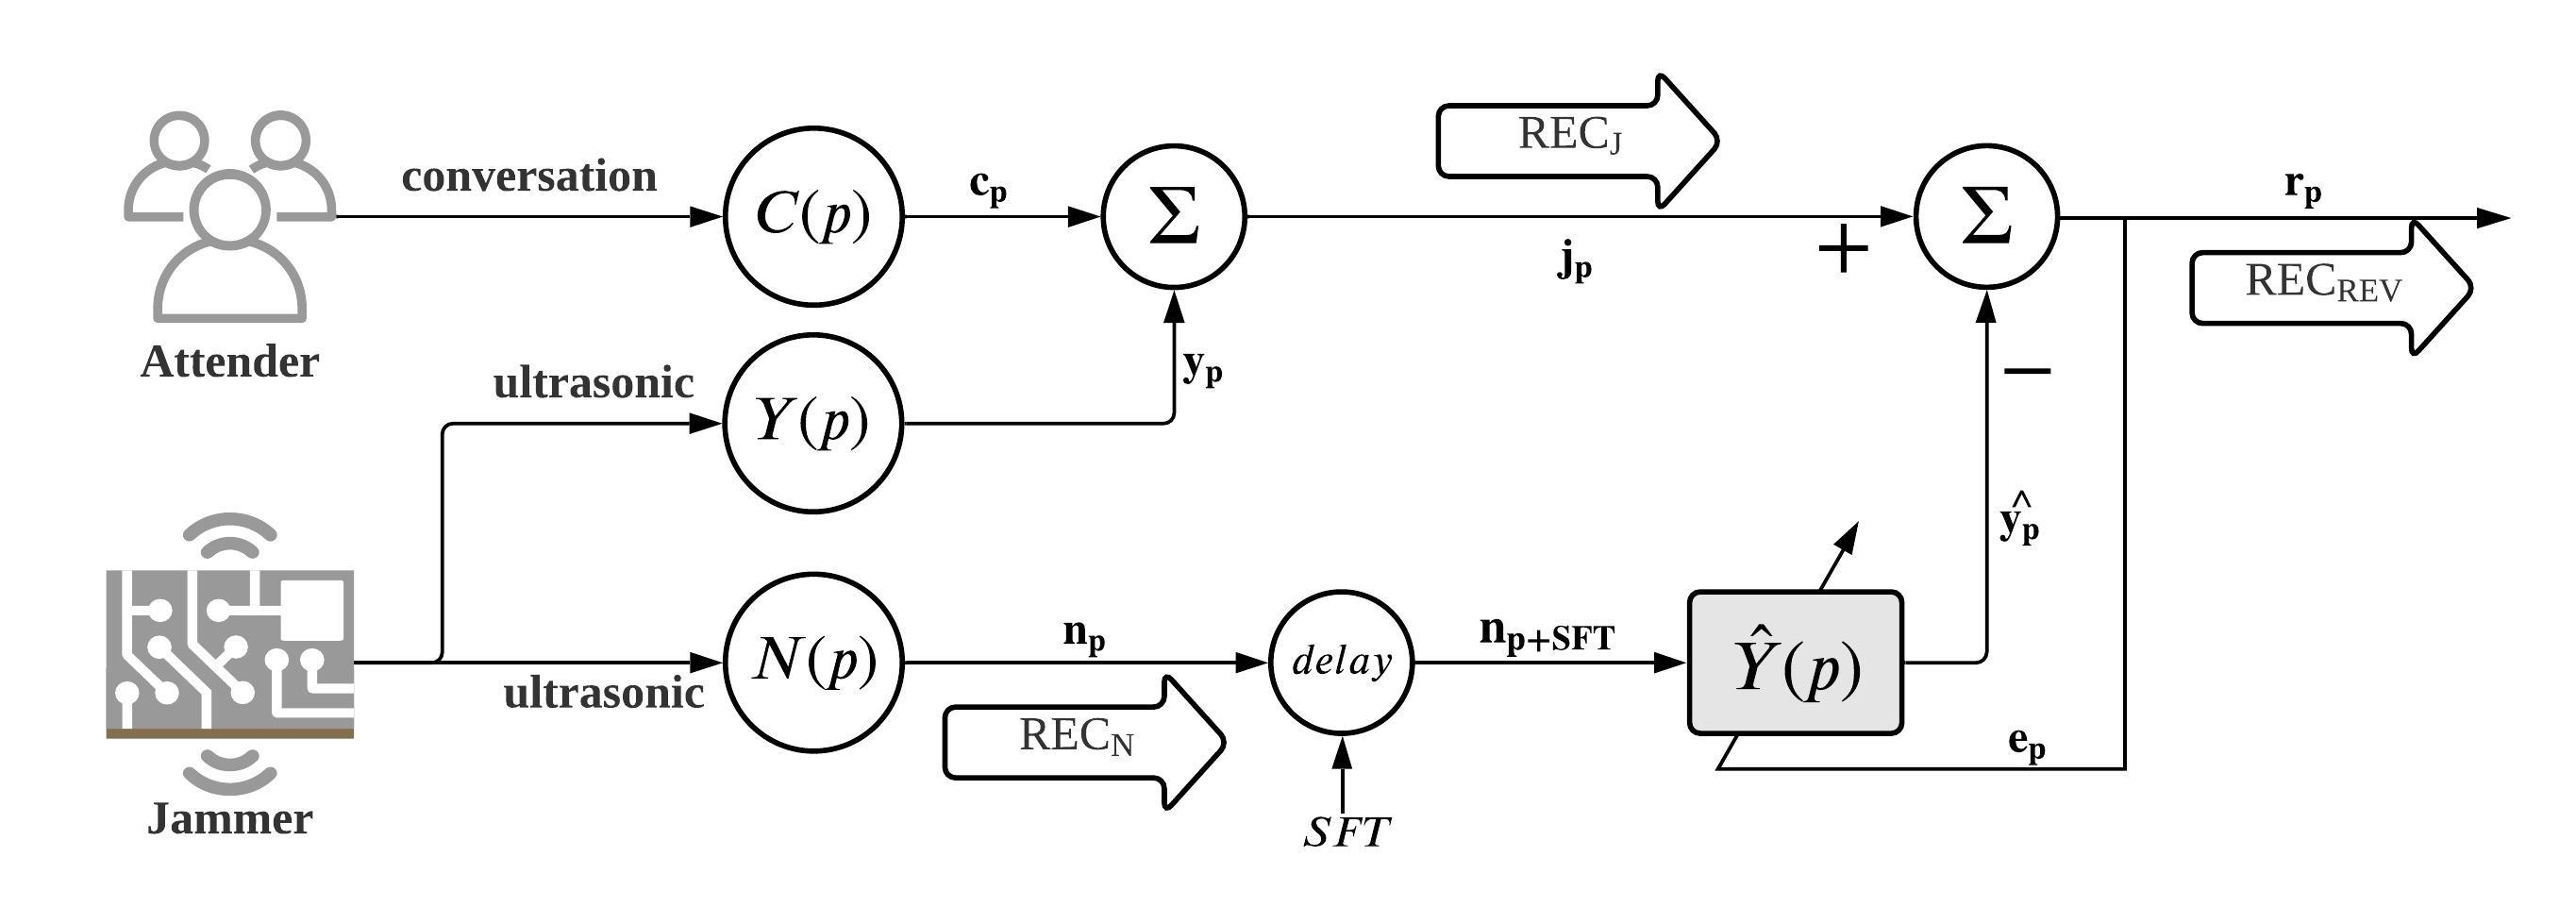
\includegraphics[width=1.0\textwidth]{anc}
    \caption{自適應噪音消除}\label{fig:anc}
\end{figure}

    受干擾的會談紀錄聲音 \DEFrecJ 由一麥克風錄製產生,此麥克風含兩個響應輸出系統,
分別定義為 \DEFfuncMicConv{\DEFpause} 與 \DEFfuncMicUSJ{\DEFpause}。
輸入 \DEFpause 為聲音於離散時間的樣本索引,用於表示響應輸出系統所在的離散時間。
\DEFfuncMicConv{\DEFpause} 為會談內容於麥克風的響應輸出函數,
其輸出定義為 \DEFmicConv,例如:會談參與者的對話聲音紀錄。
\DEFfuncMicUSJ{\DEFpause} 為純超音波麥克風干擾器於麥克風的響應輸出函數,
其輸出定義為 \DEFmicUSJ,例如:超音波麥克風干擾器產生的純噪音。
\DEFfuncMicConv{\DEFpause} 與 \DEFfuncMicUSJ{\DEFpause} 屬於同一麥克風且同時作用,
因此紀錄的聲音樣本為兩者輸出的疊加,定義為 \DEFmicRecJ $=$ \DEFmicConv $+$ \DEFmicUSJ。
且當錄音時間為 \DEFtimeREC 且取樣率為 \DEFsamplerate 時,
定義此錄音離散時間長度為 \DEFtimeLen $=$ \DEFsamplerate $\times$ \DEFtimeREC。
因此定義 \DEFrecJ $=$ $[j_{1}, ~j_{2}, ~ ...,~ j_{L}]$。

    用於產生純噪音聲音記錄 \DEFrecN 的麥克風,
對於純超音波麥克風干擾器的響應輸出系統定義為 \DEFfuncMicUSN{\DEFpause}。
輸入 \DEFpause 為聲音於離散時間的樣本索引,代表此響應輸出系統的離散時間。
\DEFfuncMicUSN{\DEFpause} 其輸出定義為 \DEFmicUSN ,例如:超音波麥克風干擾器產生的純噪音。
若噪音聲音記錄 \DEFrecN 的錄音離散時間長度為 \DEFtimeLen,
則定義 \DEFrecN $=$ $[n_{1}, ~n_{2}, ~ ...,~ n_{L}]$。

    理想上,響應輸出系統 \DEFfuncMicUSN{\DEFpause} 與 \DEFfuncMicUSJ{\DEFpause} 相同,
皆為超音波麥克風干擾器於麥克風的響應輸出函數。
因此理想上,因為 \DEFmicRecJ $=$ \DEFmicConv $+$ \DEFmicUSJ,若 \DEFmicUSJ 與 \DEFmicUSN 相等。
應可以將 \DEFmicRecJ 減去 \DEFmicUSN 產生消除噪音後的樣本定義為 \DEFmicRecREV,且應等於 \DEFmicConv。
進而獲得消除噪音後的有效會談聲音記錄 $[r_{1}, ~r_{2}, ~ ...,~ r_L]$,
定義為 $[$ \DEFmicRecREV $~|~$ \DEFmicRecREV $=$ \DEFmicRecJ $-$ \DEFmicUSN $,~  p=1~...L]$。

    但於實體場域中,可能因錄音時間、麥克風型號、距離與角度等環境因素,
兩個響應輸出系統 \DEFfuncMicUSN{\DEFpause} 與 \DEFfuncMicUSJ{\DEFpause} 之間存在差異。
根據實驗環境不同,\DEFmicRecREV 與 \DEFmicConv 可能相去甚遠,
導致此無法有效的還原產生消除噪音後的會談聲音記錄。

\subsection{方法與應用}\label{subsec:anc-prob-meth}

    為解決前節所描述的問題,透過引入兩個機制來嘗試解決。
(一)、聲音樣本的離散時間誤差對齊;
(二)、建立遞移函數,轉換純噪音聲音紀錄趨近於目標欲消去噪音;
如圖 \ref{fig:anc}。

    首先透過聲音樣本的離散時間誤差值推估函數 \DEFfuncEstm{},獲得聲音樣本的離散時間誤差值 \DEFshift。
透過消除噪音時,將輸入噪音聲音紀錄的離散時間索引值 \DEFtimeLen 加上離散時間誤差值 \DEFshift,
即可對齊修正輸入噪音聲音紀錄與欲消去噪音的離散時間誤差。
關於聲音樣本的離散時間誤差值推估函數 \DEFfuncAnc{}
將於次節 \ref{sec:estimate} \nameref{sec:estimate}中詳細說明。

    在輸入噪音聲音記錄與目標欲消除噪音兩者於離散時間數列對齊後,
若想有效提升噪音消除的效果,需使輸入噪音聲音趨近於目標欲消除噪音。
因此建立一遞移函數 \DEFfuncAf{\DEFpause},將純噪音聲音響應輸出 \DEFmicUSN 轉換為 \DEFmicUSD。
並且重新定義產生消除噪音後的樣本 \DEFmicRecREV 為 \DEFmicRecJ 減去 \DEFmicUSD。
綜上所述可以推導出,當轉換後的純噪音聲音響應輸出 \DEFmicUSD 與 \DEFmicUSJ 的差異越小時,
\DEFmicRecREV 與 \DEFmicConv 的差異也越小,即噪音消除的效果越好。

\begin{center}
\begin{tabularx}{0.55\textwidth} {>{\raggedright\arraybackslash}X}
    \DEFmicRecJ $~=~$ \DEFmicConv $~+~$ \DEFmicUSJ \\
    \DEFmicRecREV $~=~$ \DEFmicRecJ $~-~$ \DEFmicUSD $~=~$
    \DEFmicConv $~+~$ \DEFmicUSJ $~-~$ \DEFmicUSD \\
    \DEFmicRecREV $~-~$ \DEFmicConv $~=~$ \DEFmicUSJ $~-~$ \DEFmicUSD \\
    $Min($\DEFmicRecREV $~-~$ \DEFmicConv $)~=~Min($ \DEFmicUSJ $~-~$ \DEFmicUSD $)$ \\
\end{tabularx}
\end{center}

    換句話說,希望得到一遞移函數 \DEFfuncAf{\DEFpause},透過轉換純超音波麥克風干擾器的響應輸出
\DEFfuncAfHT{\DEFpause} $\cdot$ \DEFfuncMicUSN{\DEFpause},使其趨近於 \DEFfuncMicUSJ{\DEFpause}。
因此本研究所設計之系統將此遞移函數 \DEFfuncAf{\DEFpause} 設計為一自適應濾波器,
並且應用 Bernard Widrow 與 Marcian Hoff 等人所提出的最小均方濾波器(Least Mean Square Filter)
\cite{widrow1975adaptive},
如圖 \ref{fig:af}。

\begin{figure}[H]
    \centering
    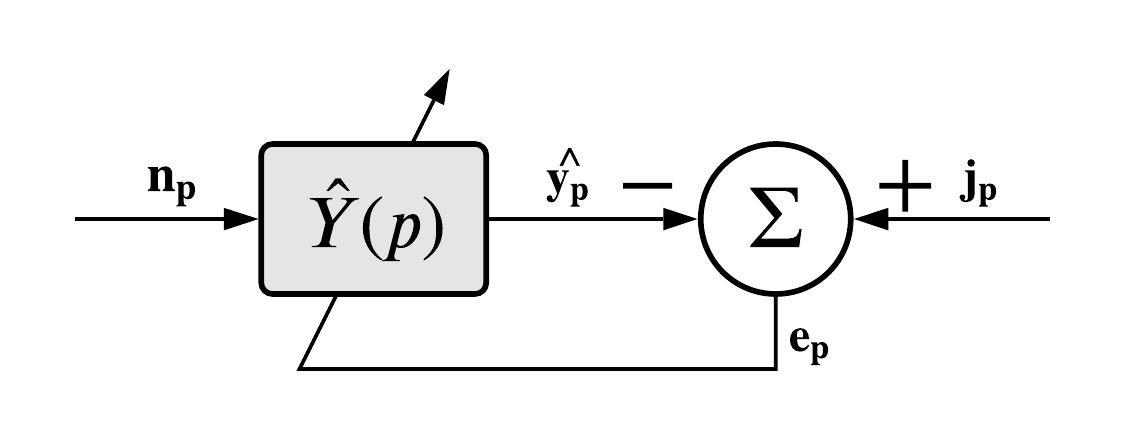
\includegraphics[width=0.45\textwidth]{af}
    \caption{自適應濾波器}\label{fig:af}
\end{figure}


\section{聲音樣本的離散時間誤差推估}\label{sec:estimate}

    本章節將說明聲音樣本的離散時間誤差值推估函 \DEFfuncEstm{}
如何推估聲音樣本的離散時間誤差值 \DEFshift,用於自適應噪音消除時對齊聲音樣本。

    在前章節中提到,本研究消於除噪音時為了提升噪音消除的成效,
透過將輸入噪音聲音紀錄 \DEFrecN 的離散時間索引值 \DEFpause 加上離散時間誤差值 \DEFshift,
來對齊修正噪音聲音紀錄 \DEFrecN 與欲消去噪音聲音紀錄 \DEFrecJ 的離散時間誤差。
已知純噪音聲音紀錄 \DEFrecN 與欲消去噪音聲音紀錄 \DEFrecJ 的取樣率 \DEFsamplerate 相同,
因此可以透過動態相對平移兩個離散時間序列來評估是否對齊,平移的量定義為 \DEFcandiSFT。

    已知由於純噪音聲音紀錄 \DEFrecN 與受干擾的會談聲音紀錄 \DEFrecJ 中的欲消去噪音,在時域上有著高度關聯性,
如圖 \ref{fig:estimate-sub} 所示。在已對齊的受干擾的聲音與純噪音,於時域上的波形表現高度相似。
且在整個離散時間序列每個樣本相減的結果(兩聲音干涉抵銷),可見能量大幅度衰減。

\begin{figure}[H]
    \centering
    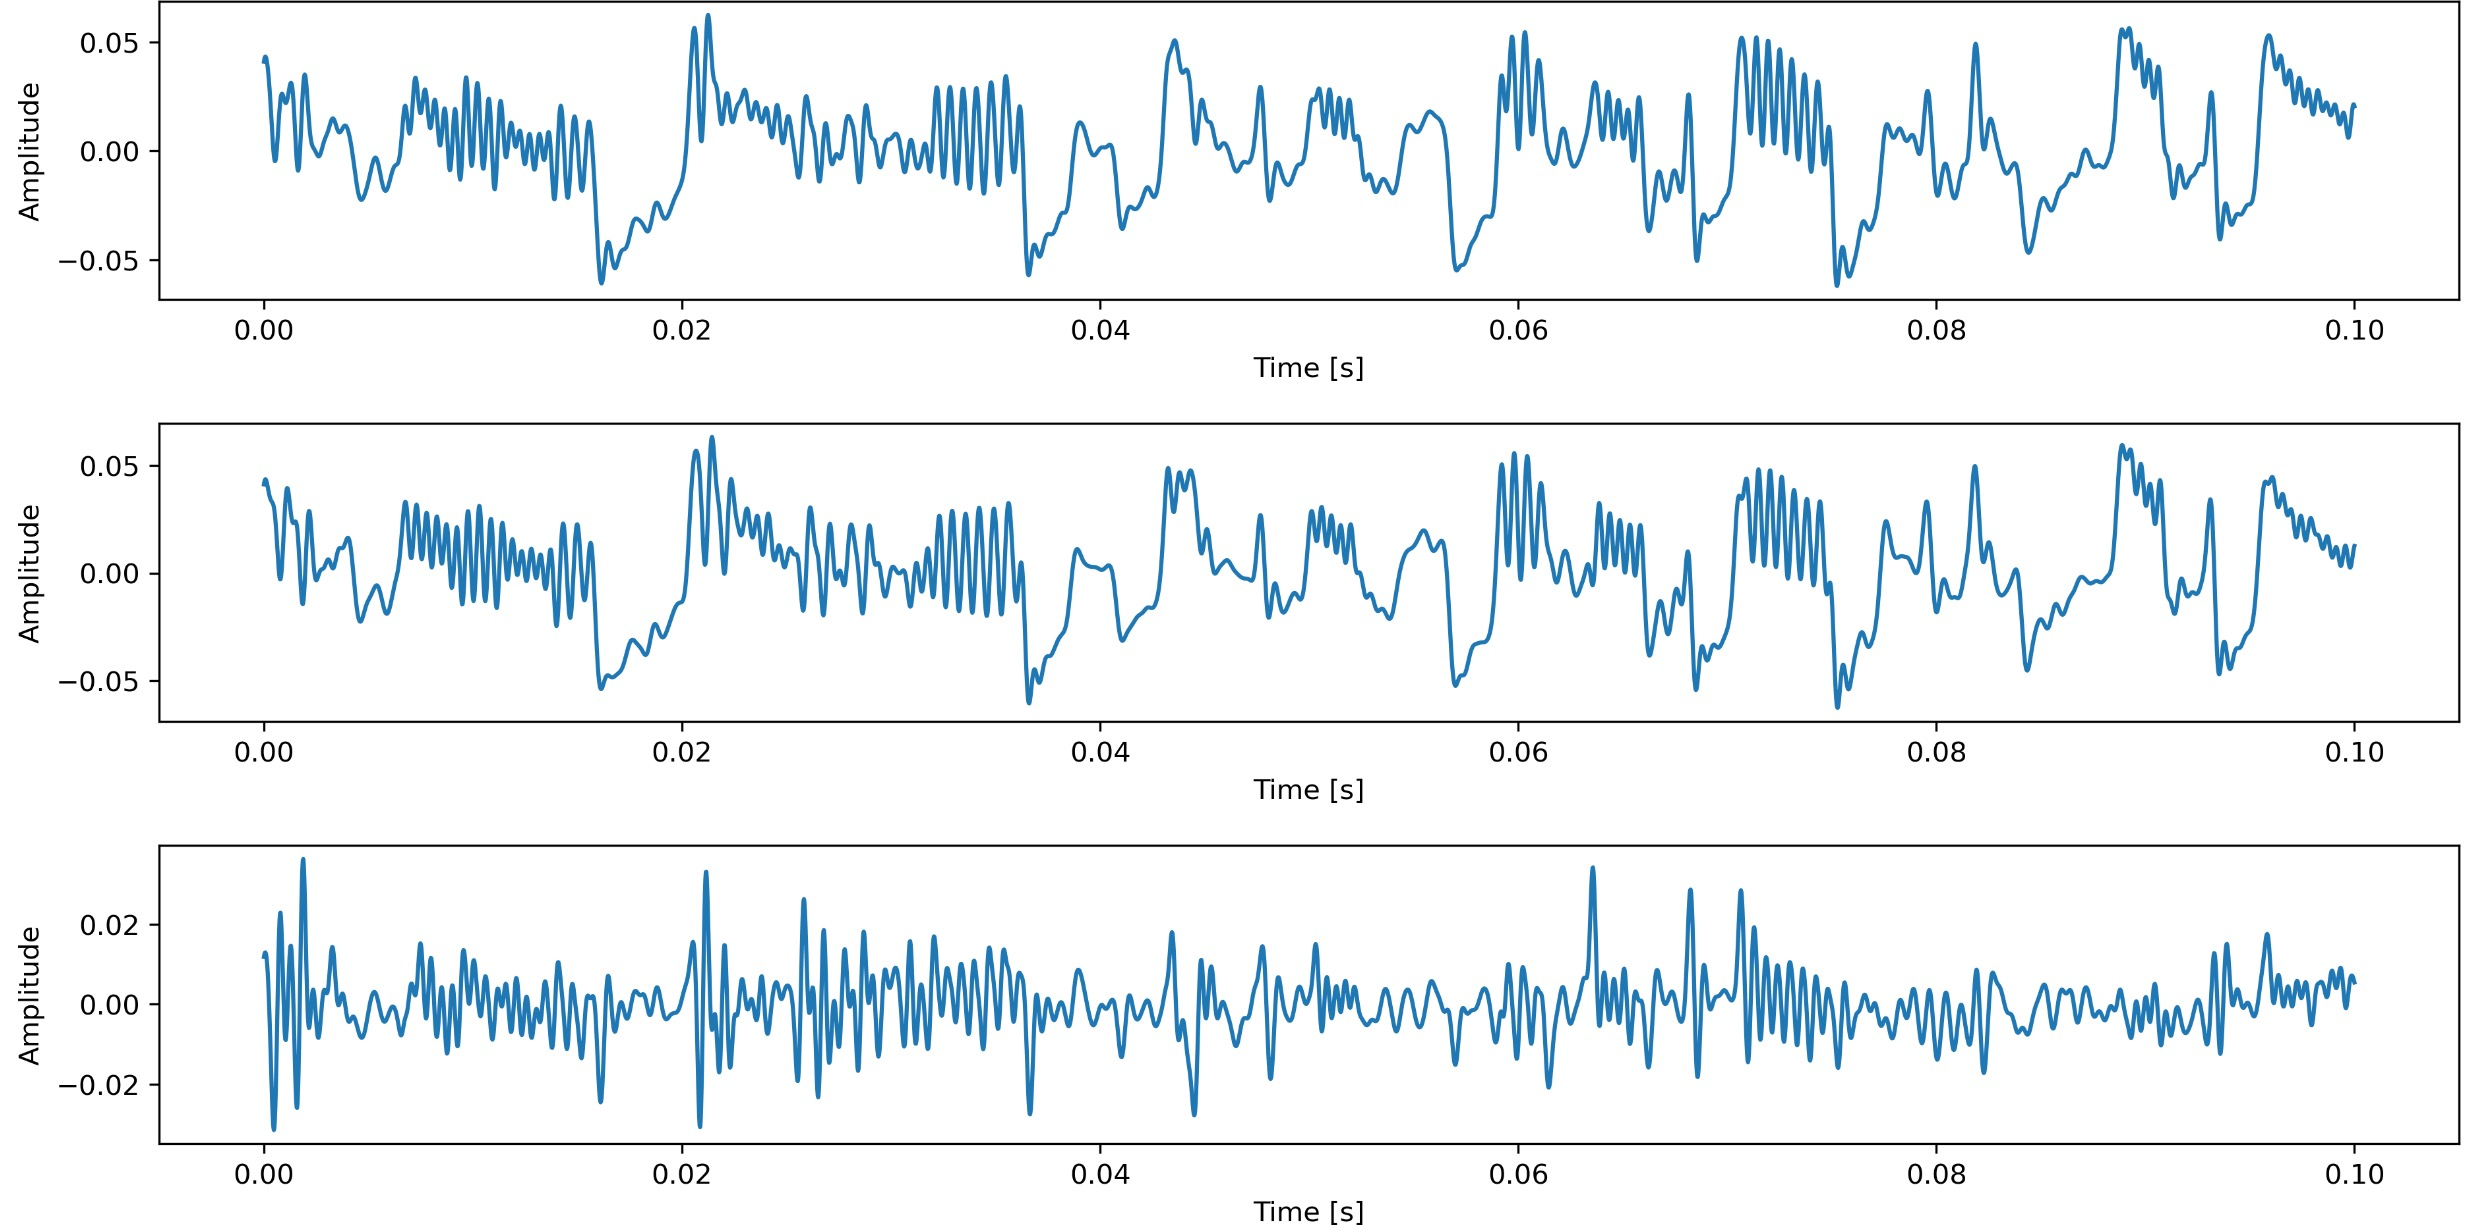
\includegraphics[width=0.9\textwidth]{sub}
    \caption{受干擾的聲音(上)與純噪音(中)干涉抵銷結果(下)}\label{fig:estimate-sub}
\end{figure}

    因此本研究提出,透過累計整個離散時間序列每個樣本相減(兩聲音干涉抵銷)後總能量差的大小,作為是否對齊的參考指標。
當找到一動態相對平移量 \DEFcandiSFT ,其干涉抵銷後總能量差為最小值,此時為對齊點。
即此時的動態相對平移量 \DEFcandiSFT,即為聲音樣本的離散時間誤差值,定義為 \DEFshift。

    兩聲音干涉抵銷後之總能量差計算演算法如圖 \ref{fig:estimate-power} 所示,其步驟如下。
首先使聲音樣本的離散時間序列索引值 \DEFpause 從零開始,逐步迭代。
在每次迭代中,將受干擾的會談聲音紀錄 \DEFrecJ 中第 \DEFpause  個樣本,
與純噪音聲音紀錄 \DEFrecN 中第 \DEFpause $+$ \DEFcandiSFT 個樣本相減,
得到第 \DEFpause 個樣本下能量差。\DEFpause 於每一次迭代逐步遞增,並累計能量差的絕對值,
至純噪音聲音紀錄 \DEFrecN 或受干擾的會談聲音紀錄 \DEFrecJ 的長度 \DEFtimeLen 停止。
最終得到特定動態相對平移量 \DEFcandiSFT 之下的累計能量差。

\begin{figure}[H]
    \centering
    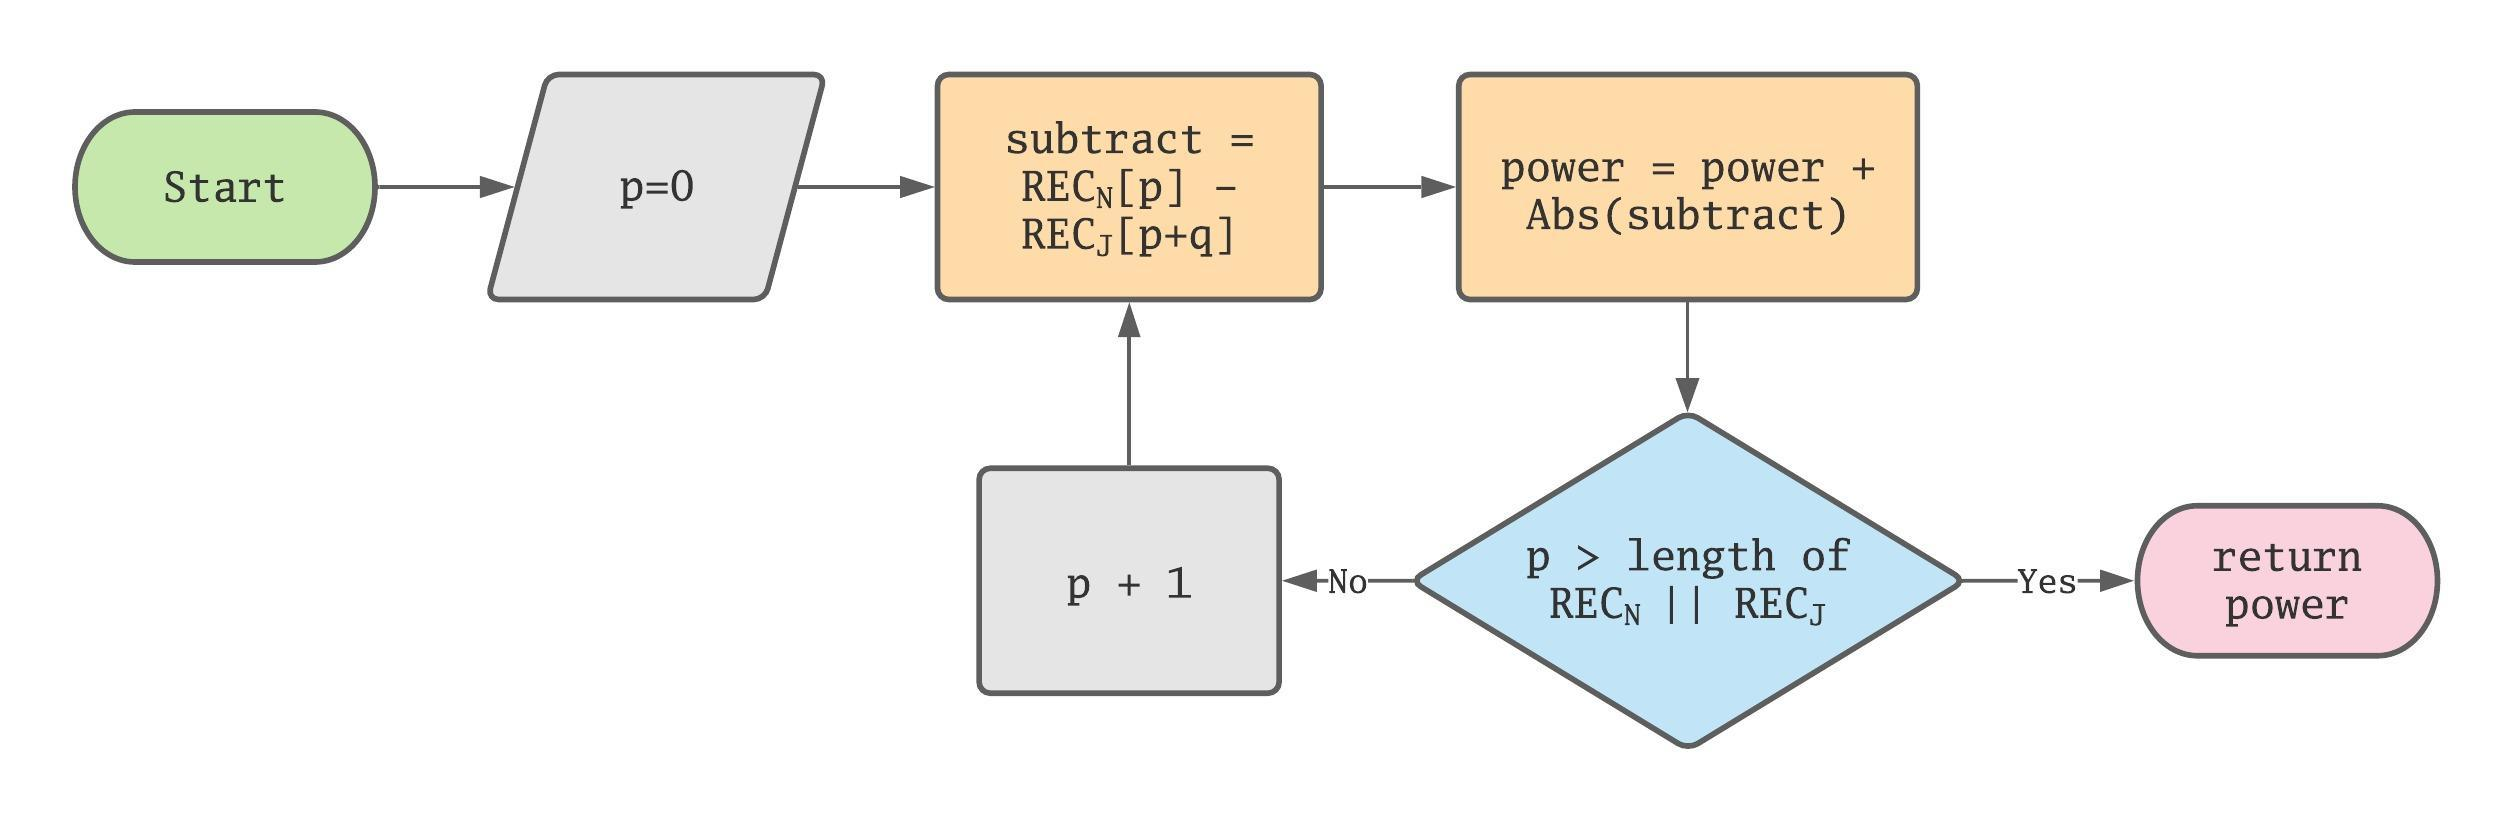
\includegraphics[width=0.95\textwidth]{estimate-shift-power}
    \caption{干涉抵銷後之總能量差計算演算法}\label{fig:estimate-power}
\end{figure}

    透過前述\nameref{fig:estimate-power},
可以計算出在特定動態相對平移量 \DEFcandiSFT 之下的累計能量差,
理想上透過歷遍所有可能的 \DEFcandiSFT,即可以找出最小的累計能量差,因而得知聲音樣本的離散時間誤差值 \DEFshift。
但若分析歷遍所有可能 \DEFcandiSFT 累計能量差的時間複雜度,會發現歷遍所有可能是沒有效率的。
分析如下:定義 $n$ 的值為離散時間序列長度 \DEFtimeLen。
計算一次特定 \DEFcandiSFT 的累計能量差,需要迭代 \DEFtimeLen 次。
又所有可能的 \DEFcandiSFT 為 $0 ~\leq$ \DEFcandiSFT $~\leq$ \DEFtimeLen。
因此當 $n$ 的值為離散時間序列長度 \DEFtimeLen 時,其時間複雜度為 $O(n^2)$。
又離散時間長度定義為 \DEFtimeLen $=$ \DEFsamplerate $\times$ \DEFtimeREC,
因此歷遍所有可能 \DEFcandiSFT 的累計能量差其時間複雜度,錄音時間長度 \DEFtimeREC 每增加一秒,
所需時間膨脹增加取樣率 \DEFsamplerate 的平方。即若取樣率 \DEFsamplerate $= 44100$,
錄音時間長度 \DEFtimeREC 每增加一秒,所需要的時間膨脹增加 $44100^2$。
故得知,透過歷遍所有可能的動態相對平移量 \DEFcandiSFT 來找出最小的累計能量差,
其時間複雜度會在錄音時間長度上,以秒為單位快速膨脹。

    為解決前述析歷遍所有可能 \DEFcandiSFT 的累計能量差效率低落的問題,
本研究提出\nameref{fig:estimate-shift},如圖 \ref{fig:estimate-shift},
其中干涉抵銷後之總能量差(Evaluation power after interference)為前述演算法 \ref{fig:estimate-power}。

\begin{figure}[H]
    \centering
    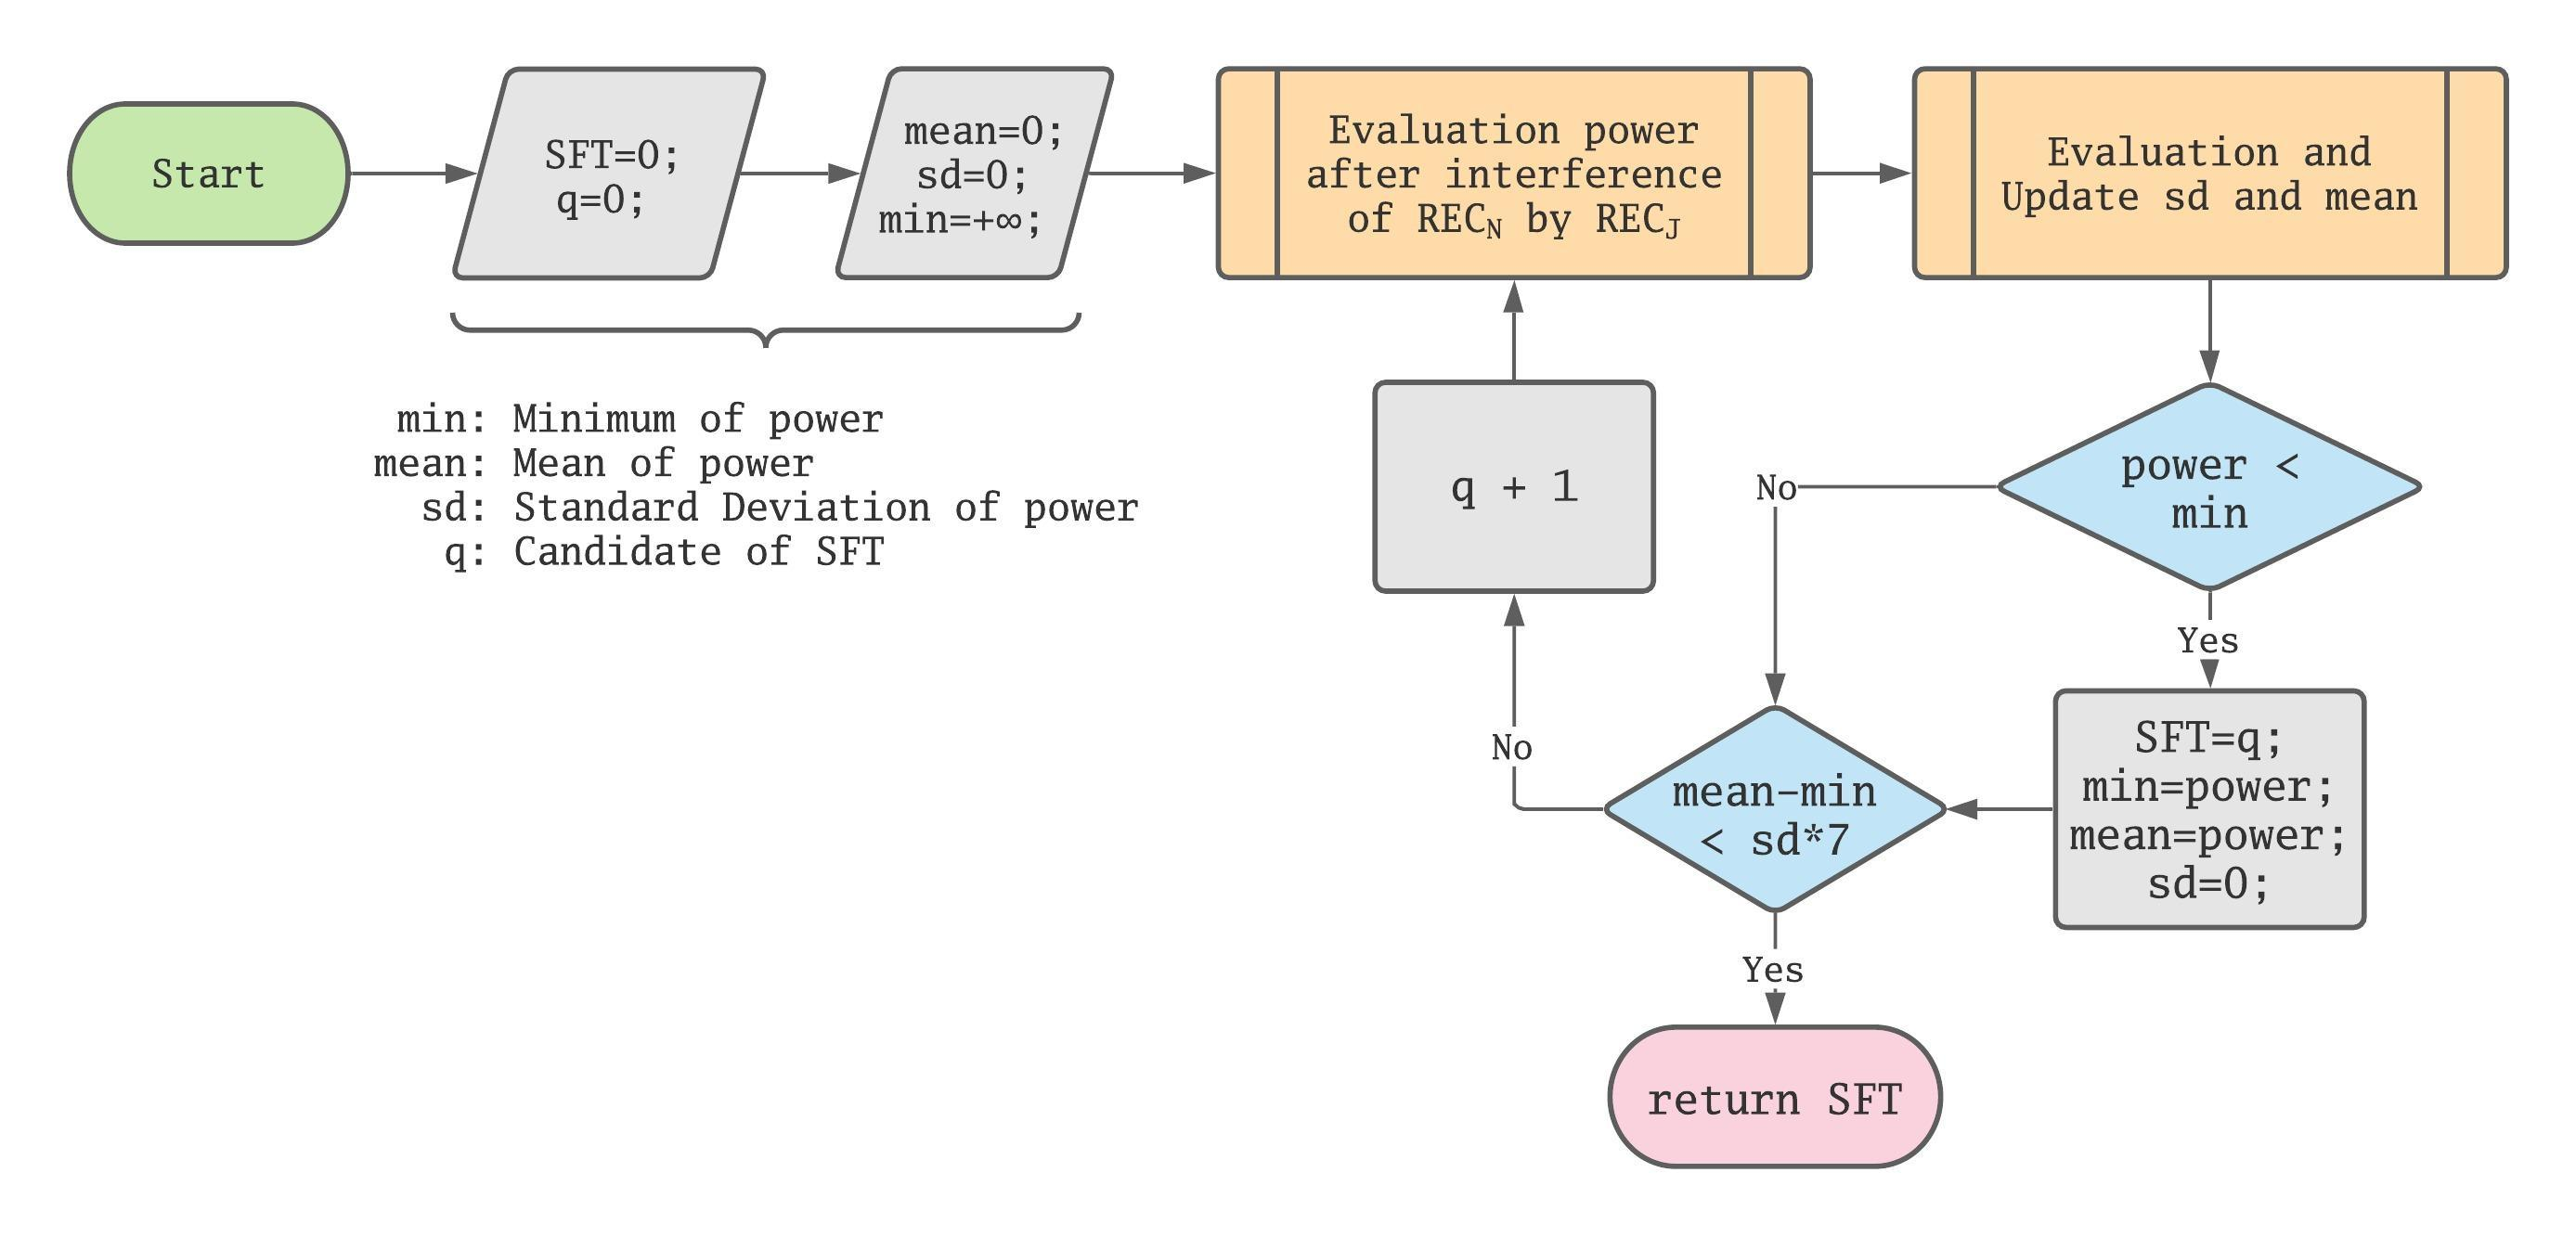
\includegraphics[width=1.0\textwidth]{estimate-shift-shift}
    \caption{聲音樣本之離散時間誤差推估演算法}\label{fig:estimate-shift}
\end{figure}

    基於前述歷遍所有可能 \DEFcandiSFT 的方法,本研究在此於每次迭代中,引入動態估計樣本標準差與平均數。
並且於每次找到新的最小累計能量差時,將樣本標準差賦值為$0$,平均數賦值為此最小累計能量差。
如此在迭代的過程中,目前已知的最小累計能量差會不斷下降,平均數會在最小累計能量差與理論整體平均之間震盪,
樣本標準差則會在$0$與母體標準差之間震盪。

    最小累計能量差在執行過程不斷更新,但我們仍未知目前最小累計能量差是否為全域最小累計能量差。
因此迭代的過程中會持續紀錄目前最小累計能量差,與計算出新的最小累計能量差時的動態相對平移量 \DEFcandiSFT。
若很長的時間都未找到新的最小累計能量差時,此時平均數會逐漸趨近理論整體平均,樣本標準差也逐漸趨近母體標準差。
此時則定義,若目前最小累計能量差與平均數相差超過 $7$ 倍樣本標準差,則演算法終止。
並且認定目前最小累計能量差,為全域最小累計能量差。而計算出目前最小累計能量差時的動態相對平移量 \DEFcandiSFT,
則為認定聲音樣本的離散時間誤差 \DEFshift,即完成此推估演算法。